As we discussed in the previous section, our motivation is to use Theorem \ref*{thm_positive_rank} to predict points of infinite order for families of elliptic curves. However, in this section we prove that in several cases the theorem will never make such a prediction. In other words, in such cases, the product 
$$\frac{\prod_i C_{E/F_i}}{\prod_j C_{E/F_j'}}$$ 
is always a norm for every subfield $\QQ(\sqrt{D})\subseteq\QQ(\rho)$. Before we give the precise statements, we give a proof of some important results that will be used throughout. The first one explicitly described the quadratic subfields of certain cyclotomic extensions.

\begin{lemma}\label{lem_subfields}
    Let $p$ be a rational prime, $n$ a positive integer and let $p^*=(-1)^{(p-1)/2}p$. Then the following holds.

    \begin{table}[!ht]
        \centering
        \begin{tabular}{|l|l|l|}
        \hline
        Cyclotomic field                    & Conditions & Quadratic subfields                   \\ \hline
        $\QQ(\zeta_{p^n})$                  & $p$ odd, any $n$    & $\QQ(\sqrt{p^*})$            \\ \hline
        \multirow{3}{*}{$\QQ(\zeta_{2^m})$} & $m=1$      & none                                  \\ \cline{2-3} 
                                            & $m=2$      & $\QQ(i)$                              \\ \cline{2-3} 
                                            & $m\geq3$   & $\QQ(i),\QQ(\sqrt{2}),\QQ(\sqrt{-2})$ \\ \hline
        \multirow{3}{*}{$\QQ(\zeta_{2^mp^n})$}  & $m=1$, $p$ odd, any $n$      & $\QQ(\sqrt{p^*})$     \\ \cline{2-3} 
                                            & $m=2$, $p$ odd, any $n$      & $\QQ(i),\QQ(\sqrt{p}),\QQ(\sqrt{-p})$                              \\ \cline{2-3}
                                            & $m\geq 3$, $p$ odd, any $n$      & $\QQ(i),\QQ(\sqrt{2}),\QQ(\sqrt{-2}),\QQ(\sqrt{p}),\QQ(\sqrt{-p}),\QQ(\sqrt{2p}),\QQ(\sqrt{-2p})$                              \\ 
                                             \hline
        \end{tabular}
        \end{table}

\end{lemma}

\begin{proof}
    Firstly, we remark that the discriminant of the field $\QQ(\sqrt{D})$, with $D$ squarefree is
    \begin{equation}
        \Delta(\QQ(\sqrt{D}))=
        \begin{cases}
            D \ \quad\text{  if } D\equiv1\pmod{4},\\
            4D \quad\text{ if } D\equiv2,3\pmod{4}.
        \end{cases}
    \end{equation}
    In addition, we also recall that $\QQ(\zeta_N)/\QQ$ is a Galois extension with $\Gal(\QQ(\zeta_N)/\QQ)=(\ZZ/N\ZZ)^*$ and that a rational prime $q$ ramifies in $\QQ(\zeta_N)/\QQ$ if and only if $q\mid N$. The result follows by combining these two properties with the Galois correspondence, as we show now.

    If $p$ is odd, then $\Gal(\QQ(\zeta_{p^n})/\QQ)=(\ZZ/p^n\ZZ)^*=C_{p^{n-1}(p-1)}$ is a cyclic group of even order, and therefore $\QQ(\zeta_{p^n})$ has one unique quadratic subfield, which can only ramify at $p$. If $p\equiv1\pmod{4}$, then the only such field is $\QQ(\sqrt{p})$ and if $p\equiv3\pmod{4}$ the only such field is $\QQ(\sqrt{-p})$. This proves the first row. 

    Since $\QQ(\zeta_2)=\QQ$ and $\QQ(\zeta_4)=\QQ(i)$, the second and third row are immediate. For $m\geq3$, $\Gal(\QQ(\zeta_{2^m})/\QQ)=(\ZZ/2^m\ZZ)^*=C_2\times C_2^{m-2}$ and therefore $\QQ(\zeta_{2^m})$ has three quadratic subfields that can only ramify at $2$. Again, it is easy to check that the only such fields are $\QQ(i)$, $\QQ(\sqrt{2})$ and $\QQ(\sqrt{-2})$, as desired. Alternatively, one can also show that $\zeta_8=(1+i)/\sqrt{2}$, which also implies the result. This proves the third row.

    The remaining rows are essentially a combination of the results we have already shown. We note that $\Gal(\QQ(\zeta_{2p^n})/\QQ)=(\ZZ/2p^n\ZZ)^*$ is cyclic while 
    $$\Gal(\QQ(\zeta_{4p^n})/\QQ)=(\ZZ/4p^n\ZZ)^*=(\ZZ/4)^*\times(\ZZ/p^n\ZZ)^*=C_2\times C_{p^{n-1}(p-1)}.$$
    Hence, $\QQ(\zeta_{2^mp^n})$ has one unique quadratic subfield if $m=1$ which must be $\QQ(\sqrt{p^*})$ and three quadratic subfields if $m=2$ which are $\QQ(i),\QQ(\sqrt{p}),\QQ(\sqrt{-p})$.
\end{proof}

The second result gives a necessary divisibility condition on primes ramifying in finite extensions of number fields. The result, however, is naturally phrased in terms of local fields.

\begin{prop}\label{prop_totally_ramified}
    Let $F/\QQ_p$ be a finite extension with residue field $\kappa$. Then there exists a tame, totally ramified cyclic extension $F_n$ of degree $n$ over $F$ if and only if $n\mid|\kappa^*|$.
\end{prop}

\begin{proof}
    Assume first that $n\mid|\kappa^*|$. Let $\pi$ be a normalizer of $F$ and consider $F_n=F(\pi^{1/n})$. We claim that $F_n$ satisfies the desired properties. Since $n\mid|\kappa^*|$, $\kappa$ contains all $n$-th roots of unity and therefore the polynomial $x^n-1$ factors into linear terms in $\kappa[x]$. The divisibility condition above implies $\Char\kappa\nmid n$ and hence by Hensel's Lemma $x^n-1$ also factors into linear terms in $F[x]$. In other words, $\QQ_p(\zeta_n)\subseteq F$ and therefore $F_n$ is the splitting field of the polynomial $x^n-\pi$. This shows that $F_n/F$ is a tame, totally ramified Galois extension, and the map 
    \begin{align*}
        \psi: \Gal(F_n/F)&\longrightarrow \mu_n\cong C_n\\
        \sigma &\longmapsto \frac{\sigma(\pi^{1/n})}{\pi^{1/n}}
    \end{align*}
    is an isomorphism of groups, which proves that the extension is cyclic of degree $n$.

    Conversely, suppose that $F_n/F$ is a tame, totally ramified cyclic extension of degree $n$. Any such field extension is generated by the $n$-th root of some uniformizer $\pi$ of $F$ (see \cite[Theorem 11.10]{Sun1}), and therefore $F_n=F(\pi^{1/n})$. The polynomial $x^n-\pi$ is Einstein over $F$, and therefore irreducible over $F$. Since $F_n/F$ is assumed to be Galois, all roots of $x^n-\pi$ lie in $F_n$. In particular, $\QQ(\zeta_n)\subseteq F_n$. Since $\Char\kappa\nmid n$, it follows that $\kappa$ also contains all $n$-th roots of unity, proving that $n\mid|\kappa^*|$ as desired. 
\end{proof}

As a consequence of this proposition, we prove one technical result about Type II or $\mathrm{II}^*$ elliptic curves over local fields $K$ admitting a $C_3$ ramified extension. We advise the reader to skip the proof by now and revisit it when this result is used later.

\begin{lemma}\label{lem_nottwo}
    Let $p\geq 5$ be a rational prime and $L_\fP/K_\fp/\QQ_p$ be finite extensions with $L_\fP/K_\fp$ Galois, ramified and $\Gal(L_\fP/K_\fp)=C_3$. Let $$E/\QQ_p:y^2=x^3+Ax+B$$ be a minimal Weierstrass equation at $\pp$ with potentially good reduction. Let $n=\nu_\pp(\Delta)$ be the valuation of the minimal discriminant. If $\gcd(n,12)=2$, then $\sqrt{\Delta}\in K_\pp$.
\end{lemma}

\begin{proof}
    The condition that $E$ has additive reduction is equivalent to $A,B\in\pp$, and the condition on ramification implies that $3\mid N(\pp)-1$ by Proposition \ref{prop_totally_ramified}. In addition, by Lemma \ref{lem_Dterms}(b), we know that $\nu_\pp(\Delta)<12$, so we need to consider two cases: $n=2$ and $n=10$, and we consider them separately. By Hensel's Lemma, $\sqrt{\Delta}\in K_\pp$ is equivalent to $\sqrt{\Delta}\in \kappa_\pp$ where $\kappa_\pp$ is the residue field of $K_\pp$. Recall that when $E$ has this simple expression, $\Delta=-16(4A^3+27B^2)$.


    \textbf{Case $n=2$:}

    In this case, $\nu_\pp(-4A^3-27B^2)=2$ and this implies that $\nu_\pp(B)=1$. Note that we also have that $A,B\in p\ZZ_p$ and therefore $\nu_p(B)=1$ and $\nu_p(-4A^3-27B^2)=2$. Let $\FF_p=\ZZ_p/p\ZZ_p$ be the residue field of $\QQ_p$. Then 
    $$\frac{-4A^3-27B^2}{p^2}\equiv -3\left(\frac{3B}{p}\right)^2\pmod{p},$$
    and hence $\sqrt{\Delta}\in\FF_p$ if and only if $\sqrt{-3}\in K_\pp$. 
    If $p\equiv1\pmod{3}$, then
    $$\left(\frac{-3}{p}\right)=\left(\frac{p}{3}\right)=1,$$
    and hence $\sqrt{\Delta}\in \FF_p\subseteq \kappa_\pp$. If $p\equiv 2\pmod{3}$, then from the condition that $3\mid N(\pp)-1$, it follows that the extension $\kappa_\pp/\FF_p$ has even degree. By the uniqueness of extensions of finite fields, it follows that $\sqrt{\Delta}\pmod{\pp}\in\kappa_\pp$ as desired.

    \textbf{Case $n=10$:} 

    In this case, $\nu_\pp(-4A^3-27B^2)=10$. When $E$ is defined by this simple expression, then $c_4=-48A$ and since $E$ is assumed to have potentially good reduction, $\nu_\pp(j)=\nu_\pp(A^3/\Delta)=3\nu_\pp(A)-10\geq 0$. Hence, $\nu_\pp(A^3)\geq12$ which implies that $\nu_\pp(-27B^2)=10$ or, equivalently, that $\nu_\pp(B)=5$. This means that $\nu_p(B)=5$ if $K_\pp/\QQ_p$ is unramified or $\nu_p(B)=1$ if $K_\pp/\QQ_p$ has ramification index $2$. In the latter case, we have that $v_p(4A^3+27B^2)=2$ and we are back to the case $n=2$. So assume that $K_\pp/\QQ_p$ is unramified. Then
    $$\frac{-4A^3-27B^2}{p^{10}}\equiv -3\left(\frac{3B}{p^5}\right)^2\pmod{p},$$
    and therefore $\sqrt{\Delta}\in\FF_p$ if and only if $\sqrt{-3}\in K_\pp$. The remaining of the proof is identical to the case $n=2$.

\end{proof}


\subsection{Notation and Preliminary Results}

In previous sections, we have discussed the behaviour of Tamagawa numbers of elliptic curves that allows us to compute them over finite extensions of number fields. The following result will be helpful to compute the local terms arising from the minimal differential in explicit examples.

    \begin{lemma}\label{lem_Dterms}
        Let $E$ be an elliptic curve over a number field $K$, $F/K$ a finite extension. Let $\pp$ be a prime in $K$ and $\fP$ a prime in $F$ above $\pp$. Let $q$ be the size of the residue field of $K$ at $\fp$. %Denote by $e_{\fP \mid \fp}$, $f_{\fP \mid \fp}$ the ramification index and residue degree of $F_{\fP} / K_{\fp}$. 

        Let $\Delta_\pp$, $\omega_{\pp}$ and $\Delta_\fP$, $\omega_{\fP}$ be the minimal discriminants and differentials for $E/K_\pp$ and $E/F_\fP$, respectively. Then the following holds.
        \begin{enumerate}[(i)]
            \setlength\itemsep{0em}
            \item If $\pp$ is unramified at $F/K$ or if $E$ has good or multiplicative reduction at $\pp$, then the minimal model of $E / K_{\fp}$ and $E / F_{\fP}$ coincide so $| \omega_{\fp} / \omega_{\fP} |_{\fP} = 1$. 
            
            \item If the residual characteristic is distinct from $2$ or $3$, and $E$ has potentially good reduction, then $v_\pp(\Delta_\pp)<12$ and the same holds for $\fP$. In particular, 
            $$\left|\frac{\omega_{\fp}}{\omega_{\fP}}\right|_{\fP} = q^{f_{\fP \mid \fp}\cdot\floor{\frac{e_{\fP\mid\fp}\nu_\fp(\Delta_\fp)}{12}}}.$$
            \item If the residual characteristic is distinct from $2$ or $3$, and $E / K_{\fp}$ has potentially multiplicative reduction then 
            $$ \left|\frac{\omega_{\fp}}{\omega_{\fP}}\right|_{\fP} = q^{f_{\fP \mid \fp} \cdot \floor{\frac{e_{\fP \mid \fp}}{2}}}.$$
        \end{enumerate}
    \end{lemma}

\begin{proof}[Proof Sketch]
    Let $e = e_{\fP \mid \fp}$, $f = f_{\fP \mid \fp}$, $\delta = v_{\fp}(\Delta_{\fp})$ and $\delta_{\fP} = v_{\fP}(\Delta_{\fP})$. Then $v_{\fP}(\Delta_{\fp}) = e n$. Thus $|\Delta_{\fp} / \Delta_{\fP} |_{\fP} = q^{f\cdot (\delta \cdot e - \delta_{\fP})}$, whence $$\left| \frac{\omega_{\fp}}{\omega_{\fP}}\right|_{\fP} = q^{f \cdot \floor{\frac{\delta \cdot e - \delta_{\fP}}{12}}}.$$ 
    \begin{enumerate}[(i)]
        \setlength\itemsep{0em}
        \setcounter{enumi}{1}
        \item If $E / K_{\fp}$ has potentially good reduction then $\delta \in \{ 2,3,4,6,8,9,10 \}$ and $\delta_{\fP} \leq 12$. By reducing to minimal Weierstrass equation for $E / F_{\fP}$ it follows that $\delta_{\fP} = \delta\cdot e - 12 \cdot \floor{\delta\cdot e / 12}$.
        
        \item Let $E / K_p$ have Kodaira type $\I_n^*$, so $\delta = 6 + n$. If $e$ is even then $E / F_{\fP}$ has Kodaira type $\I_{en}$, so $\delta_{\fP} = en$ and $\delta \cdot e - \delta_{\fP} = 6 e$.
        Else if $e$ is odd, $E / F_{\fP}$ has Kodaira type $\I_{en}^*$ so $\delta_{\fP} = 6 + en$ and $\delta\cdot e - \delta_{\fP} = 6 e - 6$. But then $\floor{(6e - 6)/12} = \floor{(e - 1)/2} = \floor{e / 2}$ since $e$ is odd.
    \end{enumerate}
\end{proof}

Following this result, we introduce some notation that will be very useful to compute the local factors $C_{E/F}$ while using the representation theoretic language discussed in Section \ref{sec_norm}.

\begin{notation}\label{not_contr}
    Let $E$ be an elliptic curve defined over $\QQ$ and let $F/K$ be a finite extension of number fields. For each finite place $\pp$ of $K$, we write the \textbf{local contribution of $\pp$} as 
    %$$T_{\mathfrak{P}\mid\pp}(E/F)=\prod_{\mathfrak{P}\mid\pp}c_\mathfrak{P}(E/F)\quad\text{and}\quad D_{\mathfrak{P}\mid\pp}(E/F)=\prod_{\mathfrak{P}\mid\pp}\left|\frac{\Delta_{E,\mathfrak{P}}^{\min}}{\Delta_E}\right|_\mathfrak{P}^{\frac{1}{12}},$$
    $$T_{\mathfrak{P}\mid\pp}(E/F)=\prod_{\mathfrak{P}\mid\pp}c_\mathfrak{P}(E/F),\quad D_{\mathfrak{P}\mid\pp}(E/F)=\prod_{\mathfrak{P}\mid\pp}\left|\frac{\Delta_{E,\mathfrak{P}}^{\min}}{\Delta_E}\right|_\mathfrak{P}^{\frac{1}{12}}$$ 
    and $C_{\fP\mid\fp}(E/F)=T_{\fP\mid\fp}(E/F)D_{\fP\mid\fp}(E/F)$, where the product ranges over primes $\fP$ of $F$ over $\pp$. 

    We are ultimately interested in computing the global contributions from the terms above, so we also introduce notation for them. With the same notation as above, we denote the \textbf{global contribution over $F$} of the Tamagawa numbers and the discriminant terms as 
    $$T(E/F)=\prod_\pp T_{\fP\mid\pp}(E/F)=\prod_\fP c_\fP(E/F)\quad\text{and}\quad D(E/F)=\prod_\pp D_{\fP\mid\pp}(E/F)=\prod_\fP \left|\frac{\Delta_{E,\mathfrak{P}}^{\min}}{\Delta_E}\right|_\mathfrak{P}^{\frac{1}{12}}.$$ 

\end{notation}

An immediate consequence of this notation is the fact that $C_{E/F}=T(E/F)D(E/F)$.
Observe that if $E$ has good reduction over $\pp$, then $T_{\mathfrak{P}\mid\pp}(E/F)=D_{\mathfrak{P}\mid\pp}(E/F)=1$ for any finite extension $F$ of $K$. 

\begin{defn}\label{not_contr_fns}
    If $G = \Gal(F / \bQ)$ then for $p \in \bQ$ we define functions $T_{\fP \mid p}$, $D_{\fP \mid p}$ and $C_{\fP \mid p}$ on $\B(G)$ by 
    \[ T_{\fP \mid p}(H) = T_{\fP \mid p}(E / F^H), \quad D_{\fP \mid p}(H) = D_{\fP \mid p}(E / F^H), \quad C_{\fP \mid p}(H) = C_{\fP \mid p}(E / F^H). \]
    Note that if $H$, $H'$ are conjugate then $F^H$, $F^{H'}$ are isomorphic, and so the values of these functions are constant on conjugate subgroups, hence they are well-defined. Define $C \colon \B(G) \to \bQ^{\times}$ by $C \colon H \mapsto C_{E / F^H}$.  
\end{defn}
    
Note that $C_{\fP \mid p}$ is a $D_p$-local function. Indeed, suppose $D_p = \Gal(F_w / \bQ_p)$, where $F_w$ denotes the completion of $F$ with respect to a place $w$ lying above $p$. For a number field $K$ and place $v$, define $$C_v(E / K) = c_v(E / K) \cdot \left| \omega / \omega_v^{\min} \right|_v.$$ We use the same notation if $K$ is a local field (then the $v$ subscript holds no meaning).
One has
\begin{equation*}
    C_{\fP \mid p} = (D_p, C_v)
\end{equation*}
where $C_v$ is a function on $\B(D_p)$ sending $H \mapsto C_v(E / F_w^H)$.

The following proposition describes these functions in the language introduced in Section \ref{sec-norm-rels} for each reduction type of $E / \bQ$. We do not attempt to write a formula for $T_{\fP \mid \fp}$ in the case of additive reduction, computing this involves using Lemma \ref{lem_add_tam}.

\begin{prop}\label{prop_local_fns}
    Let $E / \bQ$ be an elliptic curve, $G = \Gal(F / \bQ)$ and $p$ a prime of $\bQ$. Let $n = v_p(\Delta_E)$. Consider the functions $C_{\fP \mid p}$, $T_{\fP \mid p}$, and $D_{\fP \mid p}$ on $\B(G)$ defined above. Then,
    \begin{enumerate}[(i)]
        \setlength\itemsep{0em}
        \item If $E / \bQ_p$ has good reduction, $C_{\fP \mid p} = 1$,
        \item If $E / \bQ_p$ has split multiplicative reduction then $C_{\fP \mid p} = T_{\fP \mid \fp} = (D_p, I_p, e n)$,
        \item If $E / \bQ_p$ has non-split multiplicative reduction, 
        $C_{\fP \mid p} = T_{\fP \mid \fp} = \left(D_p, I_p,
        \left\{\begin{smallmatrix}
            2   & 2 \mid en, 2 \nmid f,  \\
            en   &  2 \mid f, \\
            1   & \text{else}
        \end{smallmatrix}\right.\right),$ 
        \item If $E / \bQ_p$ has potentially good reduction and $p \not= 2, 3$, $D_{\fP \mid p} = (D_p, I_p, p^{f \floor{e n /12}})$, 
        \item If $E / \bQ_p$ has potentially multiplicative reduction and $p \not= 2, 3$, $D_{\fP \mid p} = (D_p, I_p, p^{f \floor{e / 2}})$.
    \end{enumerate}  
\end{prop} 
 
\begin{proof}
    \
    \begin{enumerate}[(i)]
        \setlength\itemsep{0em}
        \item Clear. 
        \item Lemma \ref{lem_Dterms}(i) implies $D_{\fP \mid p} = 1$. If $K' / \bQ_p$ is a finite extension of ramification degree $e$, then $E / K'$ has split multiplicative reduction of type $\I_{en}$, which has Tamagawa number $en$ by Lemma \ref{lem_mult_tam}.
        \item As for split, $D_{\fP \mid p} = 1$. The description follows from applying Proposition \ref{prop_semi_red} (iii) (non-split becomes split when the residue degree is even), and Lemma \ref{lem_mult_tam}. 
        \item Follows from Lemma \ref{lem_Dterms}(ii),
        \item Follows from Lemma \ref{lem_Dterms}(iii).
    \end{enumerate}
\end{proof}
%An immediate consequence of this notation is the fact that 
%$$C_{E/F}=\prod_{\pp}C_{\mathfrak{P}\mid \pp}(F/K);$$
%that is, we can calculate $C_{E/F}$ by calculating the contribution locally at each prime of $K$. 
%{\color{red} also important to mention at some point that if the reduction is semistable, then the terms in a norm relation coming from the discriminant also vanish. Probably this would have to be introduced later.}

\begin{rem}\label{rephrase-thm}
    We rephrase Theorem \ref{thm_positive_rank} in the language introduced in $\S$\ref{sec-norm-rels}. 
    Replacing $\rho$ by the sum of its conjugates by elements of $ \Gal(\bQ(\rho) / \bQ(\sqrt{D}))$, we may assume that $\bQ(\rho) = \bQ(\sqrt{D})$. Note that this does not affect the order of $\rho$ in $\C(G)$, nor the set of $\rho$-relations (since $\repnorm{\rho}$ is unchanged). 
    
    Let $\Theta$ be a $\rho$-relation with $\bC[G / \Theta] = \repnorm{\rho}^{\oplus m}$. Let $C \colon \B(G) \to \bQ^{\times}$ be the function sending $H \mapsto C_{E / F^H}$. The theorem then states that, if $\Theta$ is not a norm relation for $C$ when $m$ is odd, or if $C(\Theta) \not\in (\bQ^{\times})^2$ for $m$ even, then $ \rk E / F > 0$. 
\end{rem}

\subsection{Cyclic Extensions}
In this section we prove the following. 
\begin{thm}\label{thm_consistent_cyclic}
    Let $d\geq2$ be a positive integer and let $F/\QQ$ be a Galois extension such that $\Gal(F/\QQ)=C_d$. Let $\chi$ be a faithful character of $C_d$ (so that $\QQ(\chi)=\QQ(\zeta_d)$) and let $\Theta_d\in B(C_d)$ be such that
    $$\CC[G/\Theta_d]=\repnorm{\chi}=\bigoplus_{\fg\in\Gal(\QQ(\zeta_d)/\QQ)}\chi^{\fg}.$$

    Let $E/\QQ$ be an elliptic curve such that
    \begin{itemize}
        \item it is semistable if $d=2^l$, or
        \item it is semistable at $2$ and $3$ if $d$ is divisible by some odd prime $q$.
    \end{itemize}

    Then for any $\QQ(\sqrt{D})\subseteq\QQ(\zeta_d)$,
    $$C(\Theta_d)\in N_{\QQ(\sqrt{D})/\QQ}(\QQ(\sqrt{D})^{\times}).$$
\end{thm}

The first step in proving Theorem \ref{thm_consistent_cyclic} is to show that the relation $\Theta_d\in B(C_d)$ exists, and to give a precise description. Recall that for each $k\mid d$ the cyclic group $C_d$ has one unique subgroup of order $k$, which is of course also cyclic. Therefore, for each $k\mid d$, there is one unique subfield $L_k$ of $F$ of degree $k$ over $\QQ$ which is also cyclic. Under the Galois correspondence, this field corresponds to the subgroup $\Gal(F/L_k)=C_{d/k}$, which has index $k$ inside $C_d$.

To give the required description, we recall that the Möbius function $\mu$ is the function supported on the square-free integers, and $\mu(n)=(-1)^s$ whenever $n$ is square free and $s$ is the number of prime factors of $n$.

\begin{lemma}\label{lem_cyclic_decomp}
    Let $E/\QQ$, $F$ and $\chi$ be as in Theorem \ref{thm_consistent_cyclic}. Writing characters of $C_d$ additively, we have that
    \begin{equation}\label{eqn_cyclic_relation}
        \fN_{\QQ(\chi)/\QQ}(\chi)=\bigoplus_{k\mid d}(\Ind_{C_k}^{C_d}\mathds{1})^{\mu(k)}.
    \end{equation}
    Furthermore, such an expression is unique, and thus
    $$\Theta_d=\sum_{k\mid d}\mu(k)C_k\in B(C_d)$$
    is the unique relation satisfying the conditions of Theorem \ref{thm_consistent_cyclic}.
\end{lemma}



\textbf{Add reference here from the exact result in the Rep Theory section.}

\begin{rem}\label{rem_radical}
    This lemma has an important consequence. Given an integer $d\geq2$, let $\rad(d)=\prod_{p\mid d}p$ be the radical of $d$, and note that a subgroup $C_k$ appears in $\Theta_d$ if and only if $C_k\leq C_{\rad(d)}$. Consequently, in terms of fields, if $L_k=F^{C_{d/k}}$ is the unique intermediate field with $[L_k:\QQ]=k$ and $K=F_{d/\rad(d)}$, then $C(\Theta_d)$ contains the local factors of $L_k$ if and only if $K\subseteq L_k\subseteq F$.

    Following this observation, we will compute $T(\Theta_d)$ and $D(\Theta_d)$ by computing locally $\Tp(C_k)$ and $\Tp(C_k)$ for each prime $\pp$ of $K$ and $k$ such that $k\mid\rad(d)$ (equivalently, for every field $L$ such that $K\subseteq L\subseteq F$), and then combinining this local information via the formula
    \begin{equation}\label{eqn_local_contr}
        T(\Theta_d)=\prod_{\pp}\Tp(\Theta_d)=\prod_\pp\left(\prod_{k\mid d} \Tp(C_k)^{\mu(k)}\right),    
    \end{equation}
    and where the same equation holds for $D(\Theta_d)$.
\end{rem}



We divide the proof of Theorem \ref{thm_consistent_cyclic} into two separate cases: odd and even cyclic extensions. The main idea in both cases is to simplify the general case into smaller cases where we can directly compute $\Cp(\Theta_d)$ for each finite place $\pp$ of $K$. Unless stated otherwise, we assume thoughout that $$\Theta_d=\sum_{k\mid d}\mu(k)C_k\in B(C_d).$$

\subsubsection{Odd Cyclic Extensions} \label{case_Cp}

For the first case, we assume that $d$ is odd. Following the observation in Remark \ref{rem_radical}, we need to calculate $\Cp(\Theta_d)$ for each finite place $\pp$ of $K=F^{C_{d/\rad(d)}}$. To that objective, we first calculate them for simple cases and then we use them for the general case. The following lemmas build on this idea.

\begin{lemma}\label{lem_Cp}
    Let $q$ be an odd rational prime, $F/K$ a Galois extension of number fields such that $\Gal(F/K)=C_q$ and $E/\QQ$ an elliptic curve with semistable reduction at $2$ and $3$. If $\Theta_q=C_1-C_q$, then 
    $$C(\Theta_q)=\frac{C_{E/F}}{C_{E/K}}$$
    is a norm from $\QQ(\sqrt{q^*})$.
\end{lemma}

\begin{proof}
    Fix some prime $\pp$ in $K$, and we calculate $\Tp(\Theta_q)\Dp(\Theta_q)$ depending on the reduction type of $\pp$. Primes $\pp$ of good reduction yield no non-trivial factors since $\Tp(\Theta_q)=\Dp(\Theta_q)=1$. Hence, we may only consider from now on primes of bad reduction. We also note since the extension $L/K$ is cyclic, the splitting behaviour of $\pp$ in $L$ is determined by the ramification index $e_\pp$ and the residual degree $f_\pp$. 
    
    If $\pp$ has multiplicative reduction, then $D_{\fP\mid\pp}(\Theta_q)=1$ and Table \ref{table_Cp} records $T_{\fP\mid\pp}(\Theta_q)$ depending on $e_\pp$ and $f_\pp$, where and the entries for split and non-split multiplicative reduction of type $\mathrm{I}_n$ are separated by a ``;''. To complete these calculations, we use repeatedly Proposition \ref{prop_semi_red} and Lemmas \ref{lem_mult_tam} and \ref{lem_add_tam}. We also use Notation \ref{not_n}.

    \begin{table}[!ht]
        \centering
        \begin{tabular}{|l|l|l|l|l|}
        \hline
        $e_\pp$ & $f_\pp$  & $T_{\fP\mid \pp}(C_q)$ & $T_{\fP\mid \pp}(C_1)$  & $\Tp(\Theta_q)$ \\ \hline
        $1$ & $1$ & $n;\tilde{n}$ & $n^q;\tilde{n}^q$ & $\square$ \\ \hline
        $q$ & $1$ & $n;\tilde{n}$ & $qn;\tilde{n}$ & $q\square;\square$ \\ \hline
        $1$ & $q$ & $n;\tilde{n}$ & $n;\tilde{n}$ & $\square$ \\ \hline
        \end{tabular}
        \caption{Contribution of semistable reduction primes in a $C_q$ extension.}
        \label{table_Cp}
    \end{table}

    Since $q$ is indeed a norm from $\QQ(\sqrt{q^*})$ by Lemma \ref{p-norm}, it follows that $\Tp(\Theta_q)$ is a norm from $\QQ(\sqrt{q^*})$ as well.

    Now assume $\pp$ has additive reduction, and let $p\ZZ=\pp\cap\QQ$. By assumption, $p\neq2,3$. Firstly, we note that $D_{\fP\mid\pp}(\Theta_q)=1$ unless $\pp$ ramifies in $F/K$, and in that case it is a power of $N_{K/\QQ}(\pp)=p^s$. If $s$ is even, then $D_{\fP\mid\pp}(\Theta_q)\in\QQss$ , so assume instead that $s$ is odd. If $L_\fP/K_\pp$ is wildly ramified, then $p=q$ is a norm from $\QQ(\sqrt{q^*})$. If $L_\fP/K_\pp$ is tamely ramified, then by Proposition \ref{prop_totally_ramified}, it follows that $q\mid p^s-1$ and therefore 
    \begin{equation}
        \left(\frac{q^*}{p}\right)=\left(\frac{p}{q}\right)=\left(\frac{p^s}{q}\right)=1
    \end{equation}
    Therefore, $p$ splits in $\QQ(\sqrt{q^*})$ and by Corollary \ref{cor_psplit_pnorm}, it follows that $p$ is a norm from $\QQ(\sqrt{q^*})$. 
    
    Finally, we compute $\Tp(\Theta_q)$. Note that since $q$ is odd, any inertia degree is odd and therefore if $\fP$ is any prime in $F$ above $\pp$, $\sqrt{D}\in K_\pp$ if and only if $\sqrt{D}\in L_\fP$ for any $D\in\QQ$. Moreover, if $q\neq 3$, then $\gcd(e_{\fP\mid\pp},12)=1$ and by Lemma \ref{lem_add_tam}, $c_\pp(E/K)=c_\fP(E/F)$. This implies that $$\Tp(\Theta_q)=c_\pp(E/K)^{\#\{\fP\mid\pp\}-1}\in\QQss$$ since the number of primes $\fP$ in $L$ above $\fp$ is odd. If $q=3$ and $\pp$ is unramified in $L/K$, then $e_{\fP\mid\pp}=1$ and the same reasoning shows that $\Tp(\Theta_q)=1$. Hence, assume $L_\fP/K_\pp$ is ramified and let $n=\nu_\pp(\Delta_{E,\pp}^{\min})$ be the valuation of the minimal discriminant of $E$ at $\pp$. By Lemma \ref{lem_add_tam}, we can obtain factors of $2$ and $3$. Since $3$ is a norm from $\QQ(\sqrt{-3})$, we only need to take care of the factors of $2$, which can only arise if $F_\fP/K_\pp$ is ramified, $\gcd(n,12)=2$ and $\sqrt{\Delta}\not\in K_\pp$. However, Lemma \ref{lem_nottwo} shows that these conditions cannot arise, and therefore $\Tp(\Theta_q)$ is a norm from $\QQ(\sqrt{-3})$ as desired.
\end{proof}


Next, we prove an analogous result for $C_{qr}$ extensions, where $q$ and $r$ are distinct odd rational primes.

\begin{lemma}\label{lem_Cpq}
    Let $q,r$ be distinct, odd rational primes and let $F/K$ be a Galois extension of number fields such that $\Gal(F/K)=C_{qr}$ and $L_k$ be the intermediate fields such that $\Gal(F/L_k)=C_{qr/k}$. Let $E/\QQ$ be an elliptic curve with semistable reduction at $2$ and $3$ and let $\Theta_{qr}=C_{qr}-C_q-C_r+C_1\in B(C_{qr})$. Then
    $$C(\Theta_{qr})=\frac{C_{E/F}C_{E/K}}{C_{E/L_q}C_{E/L_r}}\in\QQss.$$
    
\end{lemma}

\begin{proof}
    The idea of the proof is identical to Lemma \ref{lem_Cp} since in a $C_{qr}$ extension $L/K$ the splitting behaviour of a prime $\pp$ of $K$ in $L$ and all the intermediate fields is determined by $e_\pp$ and $f_\pp$. If $\pp$ has multiplicative reduction, then $\Dp(\Theta_{qr})=1$, and Table \ref{table_Cpq} records the Tamagawa numbers depending on $e_\pp$ and $f_\pp$, and again the entries for split and non-split multiplicative reduction of type $\mathrm{I}_n$ are separated by ``;''.

    \begin{table}[!ht]
        \centering
        \begin{tabular}{|l|l|l|l|l|l|l|}
        \hline
        $e_\pp$ & $f_\pp$  & $T_{\fP\mid \pp}(C_{qr})$ & $T_{\fP\mid \pp}(C_r)$ & $T_{\fP\mid \pp}(C_q)$ & $T_{\fP\mid \pp}(C_1)$ & $\Tp(\Theta_{qr})$ \\ \hline
        $1$ & $1$ & $n;\tilde{n}$ & $n^q;\tilde{n}^q$ & $n^r;\tilde{n}^r$ & $n^{qr};\tilde{n}^{qr}$ & $\square$ \\ \hline
        $1$ & $q$ & $n;\tilde{n}$ & $n;\tilde{n}$ & $n^r;\tilde{n}^r$ & $n^r;\tilde{n}^r$ & $\square$ \\ \hline
        $1$ & $r$ & $n;\tilde{n}$ & $n^q;\tilde{n}^q$ & $n;\tilde{n}$ & $n^q;\tilde{n}^q$ & $\square$ \\ \hline
        $1$ & $qr$ & $n;\tilde{n}$ & $n;\tilde{n}$ & $n;\tilde{n}$ & $n;\tilde{n}$ & $\square$ \\ \hline
        $q$ & $1$ & $n;\tilde{n}$ & $qn;\tilde{n}$ & $n^r;\tilde{n}^r$ & $q^rn^r;\tilde{n}^r$ & $\square$ \\ \hline
        $q$ & $r$ & $n;\tilde{n}$ & $qn;\tilde{n}$ & $n;\tilde{n}$ & $qn;\tilde{n}$ & $\square$ \\ \hline
        $r$ & $1$ & $n;\tilde{n}$ & $n^q;\tilde{n}^q$ & $rn;\tilde{n}$ & $r^qn^q;\tilde{n}^q$ & $\square$ \\ \hline
        $r$ & $q$ & $n;\tilde{n}$ & $n;\tilde{n}$ & $rn;\tilde{n}$ & $rn;\tilde{n}$ & $\square$ \\ \hline
        $qr$ & $1$ & $n;\tilde{n}$ & $qn;\tilde{n}$ & $rn;\tilde{n}$ & $qrn;\tilde{n}$ & $\square$ \\ \hline
        \end{tabular}
        \caption{Contribution of multiplicative reduction primes in a $C_{qr}$ extension.}
        \label{table_Cpq}
    \end{table}

    Assume instead that $\pp$ has additive reduction. It is straightforward to check that $\Tp(\Theta_{qr})$ is a rational square. Indeed, since $q$ and $r$ are distinct odd primes, we may assume that $q\neq 3$. In that case, both $L_q/K$ and $F/L_r$ are $C_q$ extensions, and from the proof of Lemma \ref*{lem_Cp}, $\Tp(C_{qr}-C_r),\Tp(C_{q}-C_1)\in\QQss$.
    
    To compute the contribution of the $\Dp$ terms, we note that by rescaling $\Delta_E$, the value of 
    $\Dp(\Theta_{qr})$
    does not change up to squares and hence we might assume that $\Delta_E=\Delta_{E,\pp}^{\min}$ and let $n=\nu_\pp(\Delta_{E,\pp}^{\min})$. Since $\Dp(\Theta_{qr})=1$ if $\pp$ is unramified in $F/K$, we assume that $\pp$ does indeed ramify. Suppose first that $e_\pp=q$, so $\pp$ is unramified in $L_r/K$. A simple calculation shows that 
    $$\Dp(C_{qr})=\Dp(C_{q})=1,\quad \Dp(C_r)=N(\pp)^{\floor{\frac{qn}{12}}}\quad\text{and}\quad \Dp(C_1)=N(\pp)^{r\floor{\frac{qn}{12}}},$$
    and therefore $\Dp(\Theta_{qr})=N(\pp)^{(r-1)\floor{qn/12}}\in\QQss$. The case $e_\pp=r$ is analogous. Finally, if $\pp$ ramifies everywhere, then a similar calculation shows that 
    $$\Dp(\Theta_{qr})=N(\pp)^{\floor{\frac{pqn}{12}}-\floor{\frac{pn}{12}}-\floor{\frac{qn}{12}}}.$$
    This may seem promising; but nevertheless the parity of the exponent only depends on $q,r,n$ modulo $12$, and for $q,r\in\{1,5,7,11\}$ (they are odd primes) and $n\in\{2,3,4,6,8,9,10\}$ (the valuation of the minimal discriminant must be relatively prime to $12$) the exponent is always even. Hence, $\Dp(\Theta_{qr})\in\QQss$, and we are done. 

    \begin{figure}[!ht]
        \centering
        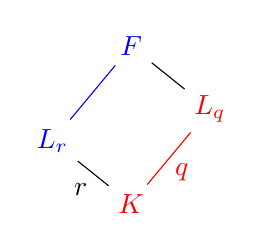
\begin{tikzpicture}

            \node [red] (Q1) at (0,0) {$K$};
            \node [red] (Q2) at (1,1.2) {$L_q$};
            \node [blue] (Q3) at (0,2) {$F$};
            \node [blue] (Q4) at (-1,0.8) {$L_r$};
        
            \draw [red] (Q1)--(Q2) node [pos=0.8, below,inner sep=0.25cm] {$q$};
            \draw (Q1)--(Q4) node [pos=0.9, below,inner sep=0.25cm] {$r$};
            \draw [blue] (Q3)--(Q4);
            \draw (Q2)--(Q3);
        
        \end{tikzpicture}
        \caption[short]{Subfields of a $C_{pq}$-extension}
    \end{figure}

    Again, the result follows immediately from the table and \eqref{eqn_local_contr}.
    
\end{proof}

We are finally ready to prove the main result of this section, from which Theorem \ref{thm_consistent_cyclic} will follow. 

\begin{lemma}\label{lem_Cd_odd}
    Let $d$ be a composite, odd squarefree integer and let $F/K$ be a Galois extension of number fields such that $\Gal(F/K)=C_{d}$. Let $E/\QQ$ be an elliptic curve with semistable reduction at $2$ and $3$ and let $L_k$ be the intermediate fields such that $\Gal(F/L_k)=C_{d/k}$. If 
    $$\Theta_d=\sum_{k\mid d}\mu(k)C_k\in B(C_d),$$
    then $C(\Theta_d)\in\QQss$.
\end{lemma}

\begin{proof}
    Let $n$ be the number of distinct prime numbers dividing $d$, so that $d=p_1\ldots p_n$ for some distinct odd primes $p_i$. We prove this result by induction. The base case for $n=2$ is the content of Lemma \ref{lem_Cpq}. Assume that the result holds for squarefree cyclic Galois extensions with $n-1$ prime factors and consider the two sets of subgroups
    $$\mathcal{A}=\{C_k:p_n\mid k\}\quad\text{and}\quad\mathcal{B}=\{C_k:p_n\nmid k\},$$
    which are clearly a partition of subgroups of $C_d$. Furthermore, the fields $\{F^{C_k}:C_k\in\mathcal{A}\}$ are precisely the intermediate fields of $L_{d/p_n}/K$, while the fields $\{F^{C_k}:C_k\in\mathcal{B}\}$ are the intermediate fields of $F/L_{p_n}$.
    Let 
    $$\Theta_\mathcal{A}=\sum_{H\in\mathcal{A}}\mu(|H|/p_n)H\quad\text{and}\quad\Theta_\mathcal{B}=\sum_{H\in\mathcal{B}}\mu(|H|)H$$
    and we note that
    \begin{equation}\label{eqn_theta}
        \Theta_d=\sum_{k\mid d}\mu(k)C_k=\sum_{p_n\nmid k\mid d}\mu(|C_k|)C_k-\sum_{p_n\mid k\mid d}\mu(|C_k|/p_n)C_k=\Theta_\mathcal{B}-\Theta_\mathcal{A}.
    \end{equation}
    Since $\Gal(L_{d/p_n}/K)=\Gal(F/L_{p_n})=C_{d/p_n}$, it follows from the inductive hypothesis applied to $L_{d/p_n}/K$ and $F/L_{p_n}$ that $C(\Theta_\mathcal{A}),C(\Theta_\mathcal{B})\in\QQss$, and therefore
    $$C(\Theta_d)=\frac{C(\Theta_\mathcal{B})}{C(\Theta_\mathcal{A})}\in\QQss,$$ 
    as desired.
    \begin{figure}[!ht]
        \centering
        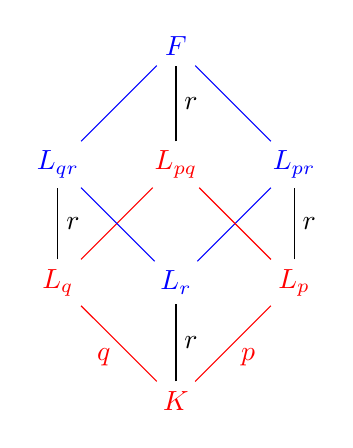
\begin{tikzpicture}

            \node [red] (Q1) at (0,0) {$K$};
            \node [red] (Q2) at (-1.5,1.5) {$L_q$};
            \node [blue] (Q3) at (0,1.5) {$L_r$};
            \node [red] (Q4) at (1.5,1.5) {$L_p$};
            \node [blue] (Q5) at (-1.5,3) {$L_{qr}$};
            \node [red] (Q6) at (0,3) {$L_{pq}$};
            \node [blue] (Q7) at (1.5,3) {$L_{pr}$};
            \node [blue] (Q8) at (0,4.5) {$F$};

            \draw [red] (Q1)--(Q2) node [pos=0.7, below,inner sep=0.25cm] {$q$};
            \draw [red] (Q1)--(Q4) node [pos=0.7, below,inner sep=0.25cm] {$p$};
            \draw (Q1)--(Q3) node [pos=0.5, right,inner sep=0.1cm] {$r$};
            \draw (Q2)--(Q5) node [pos=0.5, right,inner sep=0.1cm] {$r$};
            \draw (Q2)--(Q6) [red];
            \draw (Q3)--(Q5) [blue];
            \draw (Q3)--(Q7) [blue];
            \draw (Q4)--(Q6) [red];
            \draw (Q4)--(Q7) node [pos=0.5, right,inner sep=0.1cm] {$r$};
            \draw (Q5)--(Q8) [blue];
            \draw (Q6)--(Q8) node [pos=0.5, right,inner sep=0.1cm] {$r$};
            \draw (Q7)--(Q8) [blue];
        
        \end{tikzpicture}
        \caption[short]{Partition of $n=3$ into $n=2$. Red fields are in $\mathcal{A}$ while blue fields are in $\mathcal{B}$.}
    \end{figure}
\end{proof}

The proof of Theorem \ref{thm_consistent_cyclic} for odd $d$ is now straightforward.

\begin{proof}[Proof of Theorem \ref{thm_consistent_cyclic} for odd $d$]
    The proof is divided into two cases depending on whether $d$ is the power of a prime or not. Suppose first that $d$ is not, so that $\rad(d)$ is a squarefree \textbf{composite} number, and let $\Theta_d=\sum_{k\mid d}\mu(k)C_k\in B(C_d)$. The subgroups appearing on $\Theta_d$ are the subgroups of $C_{\rad(d)}$ and therefore by Lemma \ref{lem_Cd_odd} applied to $F/F^{C_{\rad(d)}}$, it follows that 
    $$C(\Theta_d)\in\QQss,$$ and therefore it is the norm of an element for any quadratic extension of $\QQ$. 

    If $d=q^n$ for some odd prime $q$ and $n\geq1$, then Lemma \ref{lem_cyclic_decomp} shows that $\Theta_d=C_1-C_q$ and Lemma \ref{lem_Cp} applied to $F/F^{C_q}$ proves that 
    $$C(\Theta_d)=\frac{C(C_1)}{C(C_q)}\in N_{\QQ(\sqrt{q^*})/\QQ}(\QQ(\sqrt{q^*})^{\times}).$$ 
    By Lemma \ref{lem_subfields} this is the only quadratic subfield of $\QQ(\zeta_{q^n})$, so the result follows.
\end{proof}
 
\subsubsection{Even Cyclic Extensions}
More care is required to prove Theorem \ref{thm_consistent_cyclic} for even $d$. This difficulty mainly lies in the case when $d$ is only divisible by one odd prime $q$. Consequently, we break down the proof into three distinct cases according to the number of odd prime divisors of $d$. If $d$ has more than one odd prime divisor, then the result follows without much work from Lemma \ref{lem_Cd_odd}, so we prove this first.

\begin{proof}[Proof of Theorem \ref{thm_consistent_cyclic} for even $d$ with more than one odd prime divisor]
    By Remark \ref{rem_radical}, recall that the subgroups present in $\Theta_d$ are precisely those such that $C_k\leq C_{\rad(d)}$, and so following a similar idea to Lemma \ref{lem_Cd_odd}, we define
    $$\mathcal{A}=\{C_k :2\mid k\mid\rad(d)\}\quad\text{and}\quad\mathcal{B}=\{C_k:2\nmid k\mid\rad(d)\},$$
    together with
    $$\Theta_\mathcal{A}=\sum_{H\in\mathcal{A}}\mu(|H|/2)H\quad\text{and}\quad\Theta_\mathcal{B}=\sum_{H\in\mathcal{B}}\mu(|H|)H. $$ 
    For each $k\mid d$, let $L_k=F^{C_{d/k}}$ be the unique subfield of degree $k$ over $\QQ$, and let $K=L_{d/\rad(d)}$. The fields $\{F^{C_k}:C_k\in\mathcal{A}\}$ are the intermediate fields of $L_{d/2}/K$ and the fields $\{F^{C_k}:C_k\in\mathcal{A}\}$ are the intermediate fields of $F/L_{2d/\rad(d)}$. However, note that 
    $$\Gal(L_{d/2}/K)=\Gal(F/L_{2d/\rad(d)})=C_{\rad(d)/2},$$
    and by assumption $\rad(d)$ is an odd number with more than one prime factor. Then Lemma \ref{lem_subfields} applied to $L_{d/2}/K$ and $F/L_{2d/\rad(d)}$ gives $\Theta_\mathcal{A},\Theta_\mathcal{B}\in\QQss$. The calculation in \eqref{eqn_theta} shows that $\Theta_d=\Theta_\mathcal{B}-\Theta_\mathcal{A}$ and therefore 
    $$C(\Theta_d)=\frac{C(\Theta_\mathcal{B})}{C(\Theta_\mathcal{A})}\in\QQss$$
    is the norm of any quadratic extension.

\end{proof}

If $d$ has no odd primes factors, then $d=2^l$ for some $l\geq1$. In that case, we assume in Theorem \ref{thm_consistent_cyclic} that $E$ is semistable, and the proof under this assumption is short. 

\begin{proof}[Proof of Theorem \ref{thm_consistent_cyclic} for $d=2^l$ and semistable $E$]

    If $l=1$, then $\QQ(\zeta_2)=\QQ$, and there is nothing to prove, so assume that $l\geq2$. If $\Gal(F/\QQ)=C_{2^l}$, then 
    $$C(\Theta_d)=\frac{C(C_1)}{C(C_2)}=\frac{C_{E/F}}{C_{E/L_{2^{l-1}}}},$$
    and $F/L_{2^{l-1}}$ is a $C_2$ extension. Importantly, we note that Table \ref{table_Cp} also applies for $q=2$, and therefore $\Cp(\Theta_d)$ is a rational square up to factors of $2$ for any prime $\pp$ of $L_{2^{l-1}}$. Lemma \ref{lem_subfields} shows that the only subfields of $\QQ(\zeta_{2^l})$ are $\QQ(i),\QQ(\sqrt{2})$ and $\QQ(\sqrt{-2})$, and since
    $$2=\Norm_{\QQ(i)}(1+i)=\Norm_{\QQ(\sqrt{-2})}(2)=\Norm_{\QQ(\sqrt{2})}(2+\sqrt{2}),$$
    it follows that $\Cp(\Theta_d)$ is a norm from every quadratic subfield of $\QQ(\zeta_{2^l})$, and the result follows.

\end{proof}

The remaining of this section is therefore devoted to the case when $d$ is divisible by one odd prime $q$, so $d=2^mq^n$. 
%When $d$ has this form, then $\Theta_d=C_1-C_2-C_q+C_{2q}$ and therefore fix $\Theta_d$ to have this expression for the remaining of this section. 
Recall that the quadratic subfields of $\QQ(\zeta_{2^mq^n})$ depend on whether $m=1$, $m=2$ or $m\geq 3$. Consequently, we prove three results that will be essential to prove the general version of each different case. The first covers the case $m=1$.

\begin{lemma}\label{lem_C2p}
    Let $q$ be an odd prime and let $F/K$ be a Galois extension of number fields such that $\Gal(F/K)=C_{2q}$ and let $L_k$ be the intermediate fields such that $\Gal(F/L_k)=C_{2q/k}$. Let $E/\QQ$ be an elliptic curve and let $\Theta_{2q}=C_{2q}-C_q-C_2+C_1\in B(C_{2q})$. Then
    $$C(\Theta_{2q})=\frac{C_{E/F}C_{E/K}}{C_{E/L_2}C_{E/L_q}}$$
    is a norm from $\QQ(\sqrt{q^*})$.
\end{lemma}

\begin{proof}
    Similarly to the proofs of Lemma \ref{lem_Cp} and \ref{lem_Cpq}, let $\pp$ be a prime in $K$. The splitting behaviour of a prime $\pp$ in $K$ is again determined by $e_\pp$ and $f_\pp$ and therefore if $\pp$ has multiplicative reduction $\Dp(\Theta_{2q})=1$ and the following table records $\Tp(\Theta_{2q})$.

    \begin{table}[!ht]
        \centering
        \begin{tabular}{|l|l|l|l|l|l|l|}
        \hline
        $e_\pp$ & $f_\pp$  & $\Tp(C_{2q})$ & $\Tp(C_2)$ & $\Tp(C_q)$ & $\Tp(C_1)$ & $\Tp(\Theta_{2q})$ \\ \hline
        $1$ & $1$ & $n;\tilde{n}$ & $n^q;\tilde{n}^q$ & $n^2;\tilde{n}^2$ & $n^{2q};\tilde{n}^{2q}$ & $\square$ \\ \hline
        $1$ & $q$ & $n;\tilde{n}$ & $n;\tilde{n}$ & $n^2;\tilde{n}^2$ & $n^2;\tilde{n}^2$ & $\square$ \\ \hline
        $1$ & $2$ & $n;\tilde{n}$ & $n^q;\tilde{n}^q$ & $n;n$ & $n^q;n^q$ & $\square$ \\ \hline
        $1$ & $2q$ & $n;\tilde{n}$ & $n;\tilde{n}$ & $n;n$ & $n;n$ & $\square$ \\ \hline
        $q$ & $1$ & $n;\tilde{n}$ & $qn;\tilde{n}$ & $n^2;\tilde{n}^2$ & $q^2n^2;\tilde{n}^2$ & $q\square;\square$ \\ \hline
        $q$ & $2$ & $n;\tilde{n}$ & $qn;\tilde{n}$ & $n;n$ & $qn;n$ & $\square$ \\ \hline
        $2$ & $1$ & $n;\tilde{n}$ & $n^q;\tilde{n}^q$ & $2n;1$ & $2^qn^q;1^q$ & $\square$ \\ \hline
        $2$ & $q$ & $n;\tilde{n}$ & $n;\tilde{n}$ & $2n;1$ & $2n;1$ & $\square$ \\ \hline
        $2q$ & $1$ & $n;\tilde{n}$ & $qn;\tilde{n}$ & $2n;1$ & $2qn;1$ & $\square$ \\ \hline
        \end{tabular}
        \caption{Contribution of multiplicative reduction primes in a $C_{2q}$ extension.}
    \end{table}

    Since $q$ is a norm from $\QQ(\sqrt{q^*})$, then $\Tp(\Theta_{2q})$ is also a norm. Now assume that $\pp$ has additive reduction and let $p\ZZ=\pp\cap\QQ$. We first consider the contribution of the Tamagawa numbers. Note that $L_q/K$ and $F/L_2$ are $C_q$ extensions and therefore $\Tp(\Theta_{2q})\in\QQss$ if $q\neq 3$ and a square up to factors of $3$ if $q=3$. In either case, $\Tp(\Theta_{2q})$ is a norm from $\QQ(\sqrt{q^*})$.

    Finally, we compute $\Dp(\Theta_{2q})$, whose value up to squares does not change if we reescale $\Delta_E$. Hence, we assume that $\Delta_E=\Delta_{E,\pp}^{\min}$ and let $n=\nu_\pp(\Delta_{E,\pp}^{\min})$. Under this assumption, all terms cancel unless $\pp$ ramifies in $F$. If $e_\pp=2$, then
    \begin{equation}\label{eqn_ep=2}
        \Dp(C_{2q})=\Dp(C_2)=1,\quad \Dp(C_q)=N(\pp)^{\floor{\frac{2n}{12}}}\quad\text{and}\quad \Dp(C_1)=N(\pp)^{q\floor{\frac{2n}{12}}},
    \end{equation}
    and therefore $C(\Theta_{2q})=N(\pp)^{(q-1)\floor{n/6}}$, a rational square. If $q\mid e_\pp$, then $q\mid N(\pp)-1$ by Proposition \ref{prop_totally_ramified}, and the reasoning is now identical to Lemma \ref{lem_Cp}. Write $N(\pp)=p^s$ for some $s\geq1$ and note that $\Dp(\Theta_{2q})\in\QQss$ if $s$ is even. Hence, we assume that $s$ is odd. In this case, $p=q$ if $(L_q)_\fP/K_\pp$ is wildly ramified and $p$ splits in $\QQ(q^*)$ if $(L_q)_\fP/K_\pp$ is tamely ramified. In either case, by Corollaries \ref{p-norm} and \ref{cor_psplit_pnorm}, $p$ is a norm from $\QQ(\sqrt{q^*})$, and hence so is $\Dp(\Theta_{2q})$.
    The result follows again from \eqref{eqn_local_contr}.

\end{proof}

Following this, we state and prove the analogous result for $m=2$.

\begin{lemma}\label{lem_C4p}
    Let $q$ be an odd prime and let $F/K$ be a Galois extension of number fields such that $\Gal(F/K)=C_{4q}$ and let $L_k$ be the intermediate fields such that $\Gal(F/L_k)=C_{4q/k}$. Let $E/\QQ$ be an elliptic curve with semistable reduction at $2$ and $3$ and let $\Theta_{4q}=C_1-C_2-C_q+C_{2q}$. Then 
    $$C(\Theta_{4q})=\frac{C_{E/F}C_{E/L_2}}{C_{E/L_4}C_{E/L_{2q}}}$$
    is a norm from $\QQ(i),\QQ(\sqrt{q})$ and $\QQ(\sqrt{-q})$. Moreover, $\Tp(\Theta_{4q})\in\QQss$ for any prime $\pp$ in $K$, and $\Dp(\Theta_{4q})\in\QQss$ unless $E$ has additive reduction at $\pp$ and $\pp$ is totally ramified in $F/K$.
\end{lemma}

\begin{proof}
    All fields appearing in the product are intermediate fields of $L_2$ and $F$, and $\Gal(F/L_2)=C_{2q}$. Let $\pp$ be a prime in $K$, let $\bar\pp\mid\pp$ be a prime above $\pp$ in $L_2$ and let $p\ZZ=\pp\cap\QQ$. Lemma \ref{lem_C2p} shows that if $E$ has multiplicative reduction over $\bar\pp$, $C_{\fP\mid\bar\pp}(\Theta_{4q})\in\QQss$ unless $e_{\bar\pp}=q$ and $f_{\bar\pp}=1$ over $F$. When this holds, $\bar\pp$ ramifies in $L_{2q}/L_2$ and is split in $L_4/L_2$, and this forces $\pp$ to split in $L_2/K$ too. Hence, $\pp=\bar\pp\bar\pp'$ for two \textbf{distinct} primes in $K$ that have the same local behaviour and therefore $\Cp(\Theta_{4q})=C_{\fP\mid\bar\pp}(\Theta_{4q})C_{\fP\mid\bar\pp'}(\Theta_{4q})=C_{\fP\mid\bar\pp}(\Theta_{4q})^2\in\QQss$, as desired.

    \begin{figure}[!ht]
        \centering
        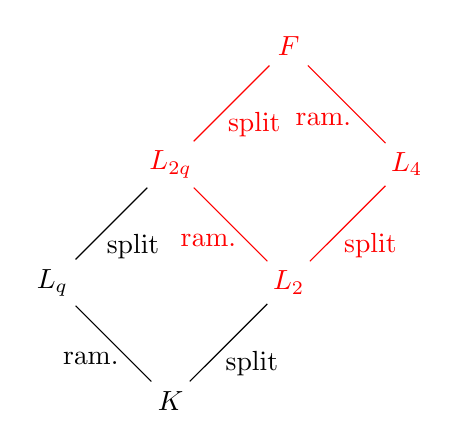
\begin{tikzpicture}

            \node (Q1) at (0,0) {$K$};
            \node (Q2) at (-1.5,1.5) {$L_q$};
            \node [red] (Q3) at (3,3) {$L_4$};
            \node [red] (Q4) at (1.5,1.5) {$L_2$};
            \node [red] (Q5) at (1.5,4.5) {$F$};
            \node [red] (Q6) at (0,3) {$L_{2q}$};
            

            \draw (Q1)--(Q2) node [pos=0.8, below,inner sep=0.4cm] {ram.};
            \draw (Q1)--(Q4) node [pos=0.8, below,inner sep=0.4cm] {split};
            \draw (Q2)--(Q6) node [pos=0.8, below,inner sep=0.4cm] {split};
            \draw [red] (Q3)--(Q5) node [pos=0.8, below,inner sep=0.4cm] {ram.};
            \draw [red] (Q4)--(Q6) node [pos=0.8, below,inner sep=0.4cm] {ram.};
            \draw [red] (Q6)--(Q5) node [pos=0.8, below,inner sep=0.4cm] {split};
            \draw [red] (Q4)--(Q3) node [pos=0.8, below,inner sep=0.4cm] {split};
        \end{tikzpicture}
        \caption[short]{\centering Field diagram for a $C_{4q}$ extension, together with the splitting\newline behaviour of a prime $\pp$ in $L_2$ with $e_\pp=q$ and $f_\pp=1$ over $F$.}
    \end{figure}

    Assume now that $E$ has additive reduction over $\bar\pp$. When $q=3$, controlling the Tamagawa numbers is lengthy, so we leave it for the end. We calculate first $\Dp(\Theta_{4q})$, which is $1$ unless $\bar\pp$ ramifies in $L/F_2$ (equivalently, $\pp$ ramifies in $L/K$). If $\pp$ is inert in $L_2/K$, then $N(\bar{\pp})\in\QQss$ and hence the size of all residues fields above $\pp$ are also squares and consequently $\Dp(\Theta_{4q})\in\QQss$ using Lemma \ref{lem_Dterms}. If $\pp=\bar\pp\bar\pp'$ splits, then $D_{\fP\mid\bar\fp}(\Theta_{4q})=D_{\fP\mid\bar\fp'}(\Theta_{4q})$, and therefore $\Dp(\Theta_{4_q})\in\QQss$ too. Finally, assume that $\pp=\bar\pp^2$ ramifies in $L_2/K$, which implies that $\bar\fp$ also ramifies in $L_4/L_2$. On the other hand, if $\bar\pp$ is unramified at $L_{2q}/L_2$, \eqref{eqn_ep=2} during the proof of Lemma \ref{lem_C2p} shows that $\Dp(\Theta_{4q})\in\QQss$ too. 

    We are therefore left with the case where $\pp$ is totally ramified in $F/K$, and Proposition \ref{prop_totally_ramified} implies that $4q\mid N(\pp)-1$. Assuming again that $\Delta_E=\Delta_{E,\pp}^{\min}$ and letting $n=\nu_{\pp}(\Delta_{E,\pp}^{\min})$, Lemma \ref{lem_Dterms} implies that 
    $$\Dp(\Theta_{4q})=N(\pp)^{\floor{\frac{n}{6}}-\floor{\frac{n}{3}}-\floor{\frac{qn}{6}}+\floor{\frac{qn}{3}}}.$$
    Again, the parity of the expression only depends on $q,n\pmod{12}$. One can easily check that for $n\in\{2,3,4,6,8,9,10\}$, the above expression is a square unless $q\equiv 3\pmod{4}$, so we assume this is the case. Write $N(\pp)=p^s$ for some $s\geq1$, which satisfies $p^s\equiv1\pmod{4q}$. If $s$ is even, then $\Dp(\Theta_{4q})\in\QQss$, so assume that $s$ is odd. Since $p^s\equiv1\pmod{4}$, this implies that $p\equiv1\pmod{4}$ and hence $p$ is a norm from $\QQ(i)$, which implies that $\Dp(\Theta_{4q})$ is a norm from $\QQ(i)$ too. Furthermore, the fact that $p^s\equiv1\pmod{4q}$ implies that
    $$\left(\frac{-q}{p}\right)=\left(\frac{q}{p}\right)=\left(\frac{p}{q}\right)=\left(\frac{p^s}{q}\right)=1,$$
    and therefore $p$ splits both in $\QQ(\sqrt{q})$ and $\QQ(\sqrt{-q})$. Since $q\equiv3\pmod{4}$, both fields have odd class number (Theorem \ref{thm_class_number}), and hence $p$ and $\Dp(\Theta_{4q})$ are norms from $\QQ(\sqrt{q})$ and $\QQ(\sqrt{-q})$ as desired. 

    Finally, we discuss Tamagawa numbers. Note that $L_{2q}/L_2$ and $F/L_4$ are $C_q$ extensions and therefore by Lemma \ref{lem_Cp} the Tamagawa numbers have a square contribution if $q\neq3$. If $q=3$, more work is required. From Lemma \ref{lem_Dterms}, we see that the Tamagawa numbers can only contribute factors of $2$ and $3$. In Lemma \ref{lem_nottwo} we showed that in $C_3$ extensions we cannot get a factor of $2$. Since $3$ is not a norm from $\QQ(\sqrt{3})$, we now need to show that we cannot get a factor of $3$ either. 
    
    We prove this result as a separate lemma, from which the result follows.    
\end{proof}

\begin{lemma}
    Let $L/K$ be a Galois extension of number fields with $\Gal(L/K)=C_{12}$ and let $L_k$ be the intermediate fields with $\Gal(F/L_k)=C_{12/k}$. Let $E/\QQ$ be an elliptic curve and let $\pp$ be a prime in $K$ not dividing $2$ or $3$ such that $E$ has potentially good reduction at $\pp$. If $\Theta_{12}=C_1-C_2-C_3+C_6\in B(C_{12})$, then $$\Tp(\Theta_{12})=\frac{\Tp(E/F)\Tp(E/L_2)}{\Tp(E/L_6)\Tp(E/L_4)}\in\QQss.$$
\end{lemma}
\begin{proof}
    Let $\bar\pp$ be a prime in $L_2$ above $\pp$ and let $n=\nu_{\bar\pp}(\Delta_{E,\bar\pp}^{\min})$ be the minimal discriminant of $E$ at $\bar\pp$. The proof is divided in three cases, depending on the splitting behaviour of $\pp$ in $L_2$. If $\pp$ splits in $L_2/K$, then $\pp=\bar\pp\bar\pp'$ where $\bar\pp$ and $\bar\pp'$ have the same local behaviour. Therefore, $T_{\fP\mid\pp}(\Theta_{12})=T_{\fP\mid\bar\pp}(\Theta_{12})T_{\fP\mid\bar\pp'}(\Theta_{12})\in\QQss$ is a square. 
    
    Next, suppose that $\pp$ is inert in $L_2/K$, which implies that $(L_2)_{\bar\pp}$ contains all square roots from $K_\pp$. This also implies that $\bar\pp$ is either inert or ramified in $L_4/L_2$. In either case, $\bar\pp$ has a unique prime $\fP$ above it in $L_4$. We note that if $\pp$ is unramified in $L_3/K$ then so is $\bar\pp$ in $L_6/L_2$ and $\fP$ in $F/L_4$ and if this holds, then by Lemma \ref{lem_Cp}
    $$\frac{\Tp(E/F)}{\Tp(E/L_4)},\frac{\Tp(E/L_6)}{\Tp(E/L_2)}\in\QQss$$
    implying $\Tp(\Theta_{12})\in\QQss$. Hence, we assume that $\pp$ is ramified in $L_3/K$. If $\bar\pp$ is inert in $L_4/L_2$, then the valuation of the minimal discriminant of $E$ at $\fP$ is also $n$ and the splitting behaviour of $\bar\pp$ in $L_6/L_2$ coincides with the splitting behaviour of $\fP$ in $F/L_4$. Hence, 
    $$\frac{\Tp(E/F)}{\Tp(E/L_4)}=\frac{\Tp(E/L_6)}{\Tp(E/L_2)},$$
    and therefore $\Tp(\Theta_{12})=1$. {\color{red} We might have a real problem if $\pp$ has $e_\pp=6$ and $f_\pp=2$. In that case, if $\gcd(n,12)=2$, then it feels that a non-trival contribution can arise.}

    Finally, assume that $\pp$ ramifies in $L_2/K$ so that $\pp=\bar\pp^2$. This immediately implies that $\bar\pp$ also ramifies in $L_4/L_2$. From Lemma \ref{lem_Cp}, we also know that in $C_3$ extensions the Tamagawa numbers above some prime contribute a square unless the prime ramifies. Hence, we may also assume that $\pp$ ramifies in $L_3/K$ and therefore $\pp$ is totally ramified in $F/K$. Using Lemma \ref{lem_add_tam}, one can easily show that the Tamagawa numbers cancel out if $\gcd(n,12)\in\{3,4,6,12\}$, so we only need to consider the case $\gcd(n,12)=2$. However, recall that $E$ has potentially good reduction at $\pp$, and since $\pp=\bar\pp^2$ ramifies, then the valuation of the minimal discriminant at $\pp$ is $n/2$ or $(n+12)/2$. But then $\gcd(\nu_\pp(\Delta_{E,\pp}^{\min}),12)=\gcd(n/2,12)=1$, a contradiction. Hence, $\Tp(\Theta_{12})\in\QQss$ as desired.
\end{proof}

Finally, we state and prove the last result, from which the case $m\geq3$ follows easily. One needs to check that the product of local factors is the norm of many quadratic subfields; thankfully, Lemma \ref{lem_C4p} has done most of work required.

\begin{lemma}\label{lem_C8p}
    Let $q$ be an odd prime and let $F/K$ be a Galois extension of number fields such that $\Gal(F/K)=C_{8q}$ and let $L_k$ be the intermediate fields such that $\Gal(F/L_k)=C_{8q/k}$. Let $E/\QQ$ be an elliptic curve with semistable reduction at $2$ and $3$ and let $\Theta_{8q}=C_1-C_2-C_q+C_{2q}$. Then 
    $$C(\Theta_{8q})=\frac{C_{E/F}C_{E/L_4}}{C_{E/L_8}C_{E/L_{4q}}}$$
    is a norm from $\QQ(\sqrt{D})$ for each $D\in\{-1,\pm2,\pm q,\pm 2q\}$.
\end{lemma}

\begin{proof}
    We prove the result locally for all primes in $L_2$. Hence, let $\bar\pp$ be a prime in $L_2$ and note that $\Gal(F/L_2)=C_{4q}$. Since the relation $\Theta_{4q}=C_1-C_2-C_q+C_{2q}\in B(C_{4q})$ has the same fixed fields as $\Theta_{8q}$, by Lemma \ref{lem_C4p}, we know that $\Tpb(\Theta_{8q})\in\QQss$ for any $\bar\pp$ and $\Dpb(\Theta_{8q})\in\QQss$ too unless $\bar\pp$ is totally ramified in $F/L_2$ and $E$ has potentially good reduction at $\bar\pp$, so assume this is the case. If $\pp=\bar\pp\cap K$, then it also follows that $\pp$ is totally ramified in $F/K$ and $E$ has potentially good reduction at $\pp$. Again, $\Dp(\Theta_{8q})$ does not change up to squares if $\Delta_{E}$ is reescaled so assume that $\Delta_{E}=\Delta_{E,\pp}^{\min}$. Under these assumptions, $\Dpb(\Theta_{8q})=\Dp(\Theta_{8q})$ is a power of $N(\pp)=N(\bar\pp)=p^s$ for some rational prime $p$ and $s\geq1$. If $s$ is even, then $\Dpb(\Theta_{8q})\in\QQss$, so assume that $s$ is odd. In addition, by Proposition \ref{prop_totally_ramified}, it follows that $p^s\equiv 1\pmod{8q}$. Since $s$ is odd and $(\ZZ/8\ZZ)^*=C_2\times C_2$, it follows that $p\equiv 1\pmod{8}$ and therefore
    \begin{equation}\label{eqn_psplitsin2}
        \left(\frac{-1}{p}\right)=\left(\frac{2}{p}\right)=\left(\frac{-2}{p}\right)=1.
    \end{equation}
    Furthermore, since $p^s\equiv1\pmod{8s}$ and $s$ is odd, then 
    \begin{equation}\label{eqn_psplitsinq}
        \left(\frac{-q}{p}\right)=\left(\frac{q}{p}\right)=\left(\frac{p}{q}\right)=1.
    \end{equation}
    Combining \eqref{eqn_psplitsin2} and \eqref{eqn_psplitsinq} together with multiplicativity of the Legendre symbol, it follows that $p$ splits in every quadratic subfield $\QQ(\sqrt{D})$ for $D\in\{-1,\pm2,\pm q,\pm2q\}$.
\end{proof}


\subsubsection*{Case 2: $d$ is divisible by one odd prime}
In this case, write $d=2^lq^n$ and let $L_k$ be the fields as above. In this case, we note that
\begin{equation}\label{eq_C2pterms}
    \frac{\prod_i C_{E/F_i}}{\prod_j C_{E/F'_j}}=\frac{C_{E/F}C_{E/L_{d/2q}}}{C_{E/L_{d/2}}C_{E/L_{d/q}}}.
\end{equation} 

If $l=1$, then we know from Lemma \ref{lem_subfields} that the only subfield of $\QQ(\zeta_{2q^n})$ is $\QQ(\sqrt{q^*})$. By Lemma \ref{lem_C2p}, it follows that \eqref{eq_C2pterms} is a norm from $\QQ(\sqrt{q^*})$, as desired.

Instead, if $l\geq2$, we consider the $C_{4q}$ extension $F/L_{d/4q}$, and all fields appearing in \eqref{eq_C2pterms} contain $L_{d/4q}$. Hence, Lemma \ref{lem_C4p} shows that the product of local terms is a norm from $\QQ(i), \QQ(\sqrt{q})$ and $\QQ(\sqrt{-q})$. By Lemma \ref{lem_subfields}, these are all quadratic subfields of $\QQ(\zeta_{2^lp^n})$, 



\subsection{Norm relations in odd order extensions}

{\color{red} add some motivation (justification) for why I'm proving this result. The point is that the test for positive rank provided by root number computations never says anything in odd order extensions. If we expect the norm relations test to be weaker than root numbers, then nor should this test.}

\begin{thm}\label{odd-exts}
 Let $E / \bQ$ be an elliptic curve, $F / \bQ$ be an extension of odd order with Galois group $G$. 
 
Assume that $E$ has semistable reduction at $2$ and $3$. 
Take any representation $\rho \in \R(G)$ with quadratic subfield $\bQ(\sqrt{D}) \subset \bQ(\rho)$ and relation
\begin{equation*}\label{odd-exp} \repnorm{\rho}^{\oplus m} =
 \left(\bigoplus_{\mathfrak{g}\in\Gal(\QQ(\rho)/\QQ)}\rho^{\mathfrak{g}}\right)^{\oplus m }=\bigoplus_i\Ind_{F_i/\QQ}\mathds{1}\ominus\bigoplus_j\Ind_{F'_j/\QQ}\mathds{1}
\end{equation*}
 as in Theorem \ref{thm_positive_rank}. Then
 \[ \frac{\prod_i C_{E/F_i}}{\prod_j C_{E/F_j'}}  \in 
    \begin{cases}
        N_{\bQ(\sqrt{D}) / \bQ}(\bQ(\sqrt{D})^{\times}) & m \ \text{odd}, \\
        \bQ^{\times 2} & m \ \text{even}.
    \end{cases} \] 
    In other words, one cannot use Theorem \ref{thm_positive_rank} to conclude that $E / F$ must have positive rank. 
\end{thm}

As in Remark \ref{rephrase-thm}, we may replace $\rho$ by the sum of its conjugates by elements of $ \Gal(\bQ(\rho) / \bQ(\sqrt{D}))$, we may assume that $\bQ(\rho) = \bQ(\sqrt{D})$. We take $D \in \bZ \ \{0,1 \}$ to be squarefree.

The product of terms we are computing is $C(\Theta)$, where $C \colon \B(G) \to \bQ^{\times}$ is given by $C \colon H \mapsto C_{E / F^H}$, and $\Theta$ is any $\rho$-relation.
We break up the function $C$ into $C = \prod_p C_{\fP \mid p} \prod_p = T_{\fP \mid p} \cdot D_{\fP \mid p}$, ranging over primes $p \in \bQ$,
as defined in Notation \ref{not_contr_fns}.
Then one has
\begin{equation*}\label{Dp-loc}
T_{\fP \mid p} \cdot D_{\fP \mid p} = (D_p, C_v)
\end{equation*}
where $C_v$ is a function on $\B(D_p)$ sending $H \mapsto C_v(E / F_w^H)$. The following result will allow us to apply some results from $\S$\ref{sec-norm-rels}.

\begin{thm}\label{odd-c-brauer}
    When $D_p$ has odd order, $C_v(\Psi) \in \bQ^{\times 2}$ for any Brauer relation $\Psi \in \B(D_p)$. 
\end{thm}

\begin{proof}
    This follows from \cite[Theorem 2.47]{reg-const} and \cite[Theorem 3.2  (Tam)]{reg-const}.
\end{proof}

\begin{cor}
It is enough to prove Theorem \ref{odd-exts} when $m$ is the order of $\repnorm{\rho}$ in $\C(G)$. Thus we need to prove that, given any $
\Theta \in \B(G)$ such that $\bC[\Theta] \simeq \repnorm{\rho}^{\oplus m}$, $\Theta$ is a norm relation for the function $C$. 
\end{cor}

\begin{proof}
    Since $\bQ(\rho)$ is quadratic, we have $\bQ^{\times 2} \subset \fieldnorm{\rho}$. As $G$ is odd, any choice of $D_p$ is odd. It follows from Theorem \ref{odd-c-brauer} that $C(\Psi) \in \bQ^{\times 2}$ for all Brauer relations $\Psi \in \B(G)$. Therefore by Proposition \ref{min-to-all}, it is enough to prove Theorem \ref{odd-exts} when $m$ is the order of $\repnorm{\rho}$ in $\C(G)$. Then $m$ divides $|G|$, hence is odd.
\end{proof}

Let $\tau$ be the generator of $\Gal(\bQ(\sqrt{D}) / \bQ)$.
Let $\ff$ be the smallest integer such that $\bQ(\sqrt{D}) \subset \bQ(\zeta_{\ff})$. Then $\ff \mid |G|$, hence is odd. By Remark \ref{conductor}, $\ff = |D|$ and that $D \equiv 1 \pmod 4$. The following shows that it is only of interest to consider decomposition groups of exponent divisible by $\ff$.

\begin{cor}\label{rational-res-2}
    Let the exponent of $D_p$ be $b$. If $\ff \nmid b$, then $(T_{\fP \mid p} \cdot D_{\fP \mid p})(\Theta) \in \bQ^{\times 2}$.
\end{cor}

\begin{proof}
    Note that $\bQ(\Res_{D_p}{\rho}) \subset \bQ(\zeta_b) \cap \bQ(\rho) \subset \bQ(\zeta_b)$. Then $\bQ(\rho) \subset \bQ(\zeta_b) \implies \ff \mid b$ by minimality of $\ff$. Since $\ff \nmid b$, we have $\bQ(\rho) \not\subset \bQ(\zeta_b)$, so $\bQ(\Res_{D_p} \rho) = \bQ$. The corollary then follows from Proposition \ref{rational-res} and Theorem \ref{odd-c-brauer}, noting that since $\C(D_p)$ is odd, multiplication by $2$ is injective. 
\end{proof}

Fix $\Theta = \sum_i n_i H_i \in \B(G)$ with $\bC[\Theta] \simeq \repnorm{\rho}^{\oplus m}$. We prove that at each prime $p$, $(T_{\fP \mid p}\cdot D_{\fP \mid p})(\Theta) \in \fieldnorm{\rho}$.  As observed, this depends on $D_p$ and $I_p$. As we deal with each local factor individually, we argue that one can take $D_p = I_p$.

\begin{lemma}\label{tam-up-to-square}
    Let $E / K$ be an elliptic curve. Let $K' / K$ be an extension of number fields odd degree, unramified at the place $v$ of $K$. Then $C_w(E / K') \equiv C_v(E / K) \mod \bQ^{\times 2}$ for any place $w$ of $K'$ with $ w \mid v$. 
\end{lemma}

\begin{proof}
This is automatic for good reduction and split multiplicative reduction. It is also clear for non-split multiplicative reduction since the residue degree cannot be even (so the reduction type remains non-split at $w$). For additive reduction, see \cite[Lemma 3.12]{reg-const}.
\end{proof}

\begin{lemma}\label{DeqI}
    At a prime $p$, we may assume that $D_p = I_p$ when computing $(T_{\fP \mid p} \cdot D_{\fP \mid p})(\Theta)$. 
\end{lemma}

\begin{proof}
Let $p$ have residue degree $f_p$. Let $L / \bQ$ be a Galois extension of degree $f_p$ with cyclic Galois group, such that $p$ is inert in $L$. Further ensure that $F \cap L = \bQ$. Then $\Gal(FL / L) = G$. Let $F_i = F^{H_i}$ and $L_i = F_i L$.

Let $v$ be a place over $p$ in $F_i$. The extension $L_i / F_i$ is Galois, so $v$ is either split or inert in $L_i$.
We claim that $C_v(E / F_i) \equiv \prod_{w | v} C_w(E / L_i) \mod \bQ^{\times 2}$. Indeed, the number of terms in the product on the right is odd, and by Lemma \ref{tam-up-to-square} $C_v(E / F_i) \equiv C_w(E / L_i) \mod \bQ^{\times 2}$. 
Letting $T_{\fP \mid p}'$ and $D_{\fP \mid p}'$ be functions on $\B(G)$ defined as in (\ref{not_contr_fns}) but with $\bQ$, $F$ replaced by $L$, $FL$, we see that $(T_{\fP \mid p} \cdot D_{{\fP \mid p}})(\Theta) \equiv (T_{\fP \mid p}' \cdot D_{\fP \mid p})(\Theta) \mod \bQ^{\times 2}$. 
Thus it is equivalent to do our computation in $FL / L$, but here $p$ has residue degree $1$.
\end{proof}

To prove Theorem \ref{odd-exts}, we proceed by considering separately each reduction type.

\subsubsection*{Good reduction}
If $E / \bQ$ has good reduction at $p$, it has good reduction at all primes lying above $p$ in subfields of $F$. Hence the Tamagawa number is always one, as well as $\left|\omega / \omega_{\fP}^{\min}\right|_{\fP}$ for any finite place $\fP \mid p$ in an intermediate field. Therefore $T_{\fP \mid p} \cdot D_{\fP \mid p} = 1$ as a  function on $\B(G)$.

\subsubsection*{Multiplicative reduction}

If $E / \bQ_p$ has multiplicative reduction, then as in the good reduction case one has $\left|\omega / \omega_{\fP}^{\min}\right|_{\fP} = 1$ for any place $\fP \mid p$ in an intermediate field. Thus $D_{\fP \mid p} = 1$.
For $T_{\fP \mid p}$, we consider non-split/split reduction separately.
\vspace{1em}

\noindent\underline{\textit{Non-split multiplicative reduction}}

Let $E / \bQ_p$ have non-split multiplicative reduction. Since $D_p = I_p$, all primes above $p$ have residue degree $1$. Then the reduction at places above $p$ remains non-split in all intermediate subfields.
It follows that 
\[ T_{\fP \mid p} = (D_p, \alpha) \]
where $\alpha$ is the constant function on $B(D_p)$ with $\alpha \in \{1, 2\}$, depending on $\ord_p(\Delta)$ being even or odd. By Proposition \ref{const-fns}, it follows that $T_{\fP \mid p}(\Theta) \in \bQ^{\times 2}$.\\  

\noindent\underline{\textit{Split multiplicative reduction}}

Now suppose $E / \bQ_p$ has split multiplicative reduction. The reduction type remains split at all places above $p$ within sub-extensions of $F / \bQ$. Let $\ord_p(\Delta) = n$. Then 
\[ T_{\fP \mid p} = (D_p, D_p, en). \]
Since the $n$ factor is constant, $(D_p, D_p, en)(\Theta) \equiv (D_p, D_p, e)(\Theta) \mod \bQ^{\times 2}$ by Proposition \ref{const-fns} .

We have $D_p = I_p = P_p \ltimes C_l$, where $P_p \triangleleft I_p$ is wild inertia, and $C_l = I_p / P_p$ is the tame quotient. $C_l$ is a cyclic group, with $l \mid p^f - 1 = p - 1$. By Corollary \ref{rational-res-2}, we may consider such $D_p$ with exponent  $p^u l$ for some $u \geq 0$ such that $\ff \mid p^u l$.

Now, $(D_p, D_p, e)(\Theta)$ is the product of ramification indices at primes above $p$. We separate the $p$-part and tame part of this expression.
Recall that the ramification index of a place $w$ above $p$ corresponding to the double coset $H_i x D_p$ has ramification degree $e_w = \frac{|I_p|}{|H_i \cap I_p^x|} =\frac{|I_p|}{|I_p \cap H^{x^{-1}}|}$.
This is the dimension of the permutation representation $\bC[D_p / D_p \cap H^{x^{-1}}]$.
Let  $D_p \cap H^{x^{-1}} = P' \ltimes C_a$ where $P' \leq P$ and $a | l$. Then the ramification index is $\frac{|P|}{|P'|}\cdot \frac{l}{a}$. 

Taking fixed points under wild inertia, one has the following isomorphism of $D_p$-representations  $$\bC[D_p / D_p \cap H^{x^{-1}}]^{P_p} \simeq \bC[D_p / P_p (D_p \cap H^{x^{-1}})] \simeq \bC[D_p / P_p \ltimes C_a].$$ This permutation representation has dimension $\frac{l}{a}$, so we've killed off the $p$-part. 
Then $$\bC[\Res_{D_p} \Theta]^{P_p} \simeq \left(\Res_{D_p} \rho^{\oplus m} \oplus \tau\left(\Res_{D_p}\rho^{\oplus m}\right)\right)^{P_p},$$
and we can consider these as representations of $D_p / P_p = C_l$.

Let $\Psi = P_p \cdot \Res_{D_p}\Theta / P_p \in B(C_l)$.
Consider the function $g$ on $B(C_l)$ with $H \mapsto [C_l : H] = \dim \bC[C_l / H]$. 
It follows from the above discussion that $(D_p, D_p, e)(\Theta)$ differs from $g(\Psi)$ up to a factor of $p$. Note that if $p = 2$ then $P_p = 1$ since $|P_p| \mid |G|$ which is odd. So we only need to consider this factor of $p$ for $p$ odd.
Crucially, this factor of $p$ doesn't matter:

\begin{lemma}
    Let $K = \bQ(\sqrt{D})$, with $\ff$ the smallest positive integer such that $K \subset \bQ(\zeta_{\ff})$. Suppose that $\ff$ is odd. Let $\ff \mid p^u l $, for some odd prime $p$, $u \geq 0$ and $l$ such that $p \equiv 1 \pmod l$. Then $p$ is the norm of an element from $K^{\times}$.
\end{lemma}

\begin{proof}
    Since $\ff$ is odd, one has $D = \prod_{q | \ff} q^*$, the product being taken over primes dividing $\ff$. Note that if $q \not= p$, then since $q \mid l$, we have $p \equiv 1 \pmod l \implies p \equiv 1 \pmod q$. By Theorem \ref{p-one-mod-disc},  $p$ is the norm of a principal fractional ideal of $K$. If $K$ is imaginary, then $p$ is the norm of an element of $K$. Else, we invoke Theorem \ref{p-norm-elem-1} or Theorem \ref{p-norm-elem-2}.
    %We show that $p$ has residue degree $1$ in the extended genus field $E^{+} = K(\{\sqrt{q^*} \colon q | \ff \})$ of $K$ ({\color{red} cf. appendix}).
    %If $q \not= p$ then $q \mid l$, so $p \equiv 1 \pmod l$. Therefore $p$ splits in any quadratic subfield of $E^{+}$ of discriminant not divisible by $p$. Else, $p$ ramifies in any quadratic subfield with discriminant divisible by $p$. Thus it is clear that $p$ has residue degree $1$ in $E^{+}$, hence also in the genus field $E$, and it follows from theorem \ref{p-principal} that $p$ is the norm of a principal ideal.  Else, we invoke theorem \ref{minus-one-norm}.
\end{proof}

Therefore we only need to worry about the tame part of our ramification indices. Let $\phi = (\Res_{D_p} \rho)^{P_p}$, viewed as a representation on $D_p / P_p = C_l$. Then $\Psi$ is a $\phi$-relation. If $\ff \nmid l$ then $\bQ(\phi) = \bQ$. Therefore $\bC[C_l / \Psi] \simeq \phi^{\oplus 2}$, implying that $\Psi = 2\Psi'$ for some $\Psi' \in \B(C_l)$ with $\bC[C_l / \Psi'] = \phi$. Then $g(\Psi) = g(\Psi')^2 \in \fieldnorm{\rho}$. Otherwise, suppose that $\bQ(\phi) = \bQ(\rho)$. It follows from Proposition \ref{index-fn-trivial} that $g(\Psi) \in \fieldnorm{\rho}$.
%has rational character. Then, arguing as in Lemma \ref{rational-res-2}, $g(\Psi) \in \bQ^{\times 2}$ {\color{red} say more?}.%Hence we may assume that $\ff \mid l$ and that $\bQ(\phi) = \bQ(\rho) = K$.

%\begin{prop}\label{semi-stable-gd}
%    One has $g(P_p \cdot \Res_{D_p}\Theta / P_p) = g(\Psi) \in \fieldnorm{\rho}$.   
%\end{prop}

%\begin{proof}
%    Write $\phi^{\oplus m} \oplus \tau(\phi^{\oplus m}) = \bC[C_l / \Psi] = \sum_{l' \mid l}{a_{l'}} \chi_{l'}$ where $a_{l'} \in \bZ$ and $\chi_{l'}$ are defined in Example \ref{cyclic-relns} (recall $\chi_{l'} = \repnorm{\varphi_{l'}}$ with $\bQ(\varphi_{l'}) = \bQ(\zeta_{l'})$ and these form a basis for the irreducible rational representations of $C_l$). Let $\Psi_{l'} = \sum_{l'' | l'}\mu(l' / l'')\cdot C_{l / l''}$ so that $\bC[\Psi_{l'}] = \chi_{l'}$, as observed in the example. Then $\bC[\Psi] \simeq \bC[\sum_{l' | l } a_{l'} \Psi_{l'}]$ which implies that $\Psi = \sum_{l' | l } a_{l'} \Psi_{l'}$ since cyclic groups have no Brauer relations.

 %   Evaluating $g$ on $\Psi_{l'}$ is trivial unless $l' = q^a$ for some $q$ prime, $a \geq 1$. Indeed, if $l' = p_1^{e_1} \cdots p_r^{e_r}$ , with $r \geq 2$ and $e_i \geq 1$, then
 %   \[ \prod_{l'' \mid l'} (l'')^{\mu(l' / l'')} = \prod_{j_1, \ldots j_r \in \{0,1\}^r } \left(p_1^{e_1 - j_1} \cdots p_r^{e_r - j_r}\right)^{\# j_i = 1} = \prod_{i = 1}^r \left(\frac{p_i^{e_i}}{p_i^{e_i - 1}}\right)^{\sum_{ j = 0}^{r - 1} \binom{r-1}{j} (-1)^j} = 1. \]
 %   On the other hand,
  %  \[ \prod_{l' \mid q^a} (l')^{\mu(q^a / l')} = q .\]
    
   % We claim that $\ff \nmid l'$ implies $a_{l'}$ is even. The irreducible representations of $C_l$ over $\bQ(\phi)$ are given by the orbits of the complex irreducible characters of $C_l$ acted upon by $H = \Gal (\bQ(\zeta_l) / \bQ(\phi))$. If $ \ff \nmid l'$ then $\bQ(\phi) \not\subset \bQ(\zeta_{l'})$, so that $B = \Gal(\bQ(\zeta_l) / \bQ(\zeta_{l'})) \not\leq H$. Then $\bQ(\phi) \cap \bQ(\zeta_{l'}) = \bQ$ so $BH = \Gal(\bQ(\zeta_l) / \bQ)$. The orbit of $\varphi_{l'}$ under $H$ is fixed by $BH$, hence is rational. It follows that $\langle \phi, \varphi_{l'} \rangle = \langle \tau(\phi) , \varphi_{l'} \rangle$ so that $a_{l'}$ is even.  

  %  Thus we can only possibly get something interesting if $\ff = q$ is a prime. But then $q$ is a norm from $\bQ(\sqrt{q^*})$ by Corollary \ref{p-norm}. 
%\end{proof}

\subsubsection*{Additive reduction}

Now suppose that $E / \bQ_p$ has additive reduction. In this case, assume that $p \geq 5$. We have $D_p = P_p \ltimes C_l$ with $ l \mid p - 1$.  
%is at worst tamely ramified in $F / \bQ$. This ensures that $D_p = I_p = C_l$ is cyclic, and $l \mid p - 1$. 
Once again we may assume that $\ff \mid p^k l$ where $p^k l $ is the exponent of $D_p$ by Corollary \ref{rational-res-2}.

Let $\delta = \ord_p(\Delta_E)$. Consider a place $\fP$ of $F^H$ over $p$ with ramification degree  $e_{\fP}$ over $\bQ$. Then $\Delta_E$ has valuation $n e_{\fP}$ with respect to $\fP$. Then $\left| \Delta_E / \Delta_{E, \fP}^{\min} \right|_{\fP} = p^{-(\delta\cdot e_{\fP} - \delta_H)}$, where $\delta_H = \ord_{\fP}(\Delta_{E, \fP}^{\min})$.
Recall that
\[ \left| \frac{\omega}{\omega_{\fP}^{\min}} \right|_{\fP}^{-12} = \left| \frac{\Delta_E}{\Delta_{E, \fP}^{\min}} \right|_{\fP} .\] 
Therefore $\left| \omega / \omega_{\fP}^{\min} \right|_{\fP} = p^{\floor{\frac{\delta\cdot e_{\fP} - \delta_H}{12}}}$.

Suppose that $E / \bQ_p$ has Kodaira type $I_n^*$, so $\delta = 6 + n$. For a finite extension $K' / \bQ_p$ with ramification degree $e$, $E / K'$ has Kodaira type $I_{en}^*$ if $e$ is odd, and type $I_{en}$ if $n$ is even. Thus in odd degree extensions the reduction type will stay potentially multiplicative. Then $\delta \cdot e_{\fP} - \delta_H = 6 e_{\fP}$.

If $E / \bQ_p$ has potentially good reduction then $\delta \in \{2,3,4,6,8,9,10 \}$. $E$ also has potentially good reduction at the place $\fP$ in $F^H$. Hence $\delta_H \leq 12$ and it follows that $\delta_H = \delta \cdot e_\fP - 12 \cdot \floor{\delta \cdot e_\fP /12}$.

In conclusion, 
\[ D_{\fP \mid p} = 
    \begin{cases}
        (D_p, D_p,\ p^{\floor{e_ /2}}) & \text{if } E \text{ has potentially multiplicative reduction}, \\
        (D_p, D_p,\ p^{\floor{\delta \cdot e/12}}) & \text{if } E \text { has potentially good reduction}.
    \end{cases}
    \]

In either case, $D_{\fP \mid p}(\Theta) \in N_{\bQ(\rho) / \bQ}(\bQ(\rho)^{\times})$. Indeed, this takes values $1$ or $p$ in $\bQ^{\times} / \bQ^{\times 2}$. But $p \equiv 1 \pmod l$ implies $p \equiv 1 \pmod \ff$ so that $p$ is the norm of a principal ideal in $\bQ(\rho)$, and hence the norm of an element, by Corollary \ref{p-one-mod-disc} and Theorem \ref{p-norm-elem-1}.

%\[ \left|\frac{\Delta_{E}}{\Delta_{E, w}^\min} \right|_w = p^{f_w 12 \cdot \floor{e_w n / 12}} \implies 
%       \left|\frac{\omega}{\omega_{w}^\min} \right|_w = p \]
\vspace{1em}

For the Tamagawa number computations, we use the description from \cite{reg-const} for computing Tamagawa numbers, as detailed in Lemma \ref{tamagawa-num}. {\color{red} maybe add a small reminder}

Firstly, suppose that $E / \bQ_p$ has reduction type $I_{n}^{*}$. 
Write $D_p = \Gal(F_w / \bQ_p)$. Since we assume $D_p = I_p$, i.e. the residue degree is one, it follows that any subextension $L'$ of $F_{w} / \bQ_p$ satisfies $\sqrt{B} \in L' \iff \sqrt{B} \in \bQ_p$ and $\sqrt{\Delta} \in L' \iff \sqrt{B} \in \bQ_p$. 
Therefore $T_{\fP \mid p} = (D_p, \alpha)$ where $\alpha \in \{2, 4\}$. But then $(D_p, \alpha)(\Theta) \in \bQ^{\times 2}$ by Proposition \ref{const-fns}.

Now suppose that $E / \bQ_p$ has potentially good reduction. Observe that in a totally ramified extension of degree coprime to $12$, the Tamagawa number remains the same. Hence for $D_p$ odd, if $3 \nmid |D_p|$ it follows that $T_{\fP \mid p} = (D_p, \alpha)$ for some constant $
\alpha$ and so $T_{\fP \mid p}(\Theta) \in \bQ^{\times 2}$.

Thus we assume that $3 \mid |D_p|$. Since we assumed $p \geq 5$, we have $D_p = I_p = P_p \ltimes C_l$ with $3 \mid l$ and $p \equiv 1 \pmod l$. 
If we have type $III$ or $III^*$ or $I_0^*$ then the Tamagawa number is still unchanged in any totally ramified extension of odd degree extension, even when the degree is divisible by $3$. We will treat the other cases separately: 

\vspace{1em}

\noindent\underline{\textit{Type $II$ and $II^*$ reduction:}}

Suppose $\delta = 2$, that is we have Type $II$ reduction. If $L' / \bQ_p$ is an odd degree extension that is divisible by $3$, then $E / L'$ has reduction type $I_0^*$. By Lemma \ref{tamagawa-num} the Tamagawa number of $E / L'$ then depends on whether $\sqrt{\Delta} \in \bQ_p$. Since we have additive reduction, we know that $p \mid A$, $p \mid B$. Moreover, $\delta = 2$ implies that $v_p(B) = 1$. Then, $\Delta = p^2\cdot \alpha$, and $\alpha \equiv -27\cdot\square \pmod p$. Therefore $\sqrt{\Delta} \in \bQ_p \iff -3$ is a square $\pmod p$. But this is the case; we assumed $p \equiv 1 \pmod l$, so $p \equiv 1 \pmod 3$. Then $\legendre{-3}{p} = \legendre{p}{3} = 1$. Therefore the Tamagawa number will be $1$ or $4$, which is a square.
On the other hand if $L' / \bQ_p$ is an extension of odd degree then the reduction type over $L'$ is $II$ or $II^*$ and the Tamagawa number is $1$. It follows that $T_{\fP \mid p}(\Theta)$ is a product of square terms, so is itself square. 

If $\delta = 10$, then $E / L'$ has reduction type $I_0^*$ whenever $3 \mid [ L' : \bQ_p]$. Once more, $v_p(A)$, $v_p(B) \geq 1$, and $v_p(\Delta) = 10 = \min(3 v_p(A), 2 v_p(B)) \implies v_p(B) = 5$. Therefore we get $\Delta = p^{10} \cdot \alpha$ with $\alpha \equiv -27\cdot\square \pmod p$, and we conclude as above.

\vspace{1em}

\noindent\underline{\textit{Type $IV$ and $IV^*$ reduction:}}

Now, if $E /\bQ_p$ has additive reduction of type $IV$ or $IV^*$, it attains good reduction over any totally ramified cyclic extension of degree divisible by $3$. This could result with $3$ coming up an odd number of times in $T_{\fP \mid p}(\Theta)$, when $\sqrt{B} \not\in \bQ_p$. 
%We show that for both types, one has $\sqrt{B} \in \bQ_p$. 
%Indeed, if $\delta = 4$, then $v_p(B) = 2$, and $v_p(A) \geq 2$. 
%\vspace{1em}
%In summary, 
%\begin{equation}
 %   \prod_{d ' \mid d} C(E / F_{\fp}^{D_{d'}})^{\mu(d / d')}
  %  = 
   % \begin{cases}
    %    1 & 3 \nmid d, \\
    %   1 & 3 \mid d, \delta \in \{0, 3, 6, 9\}, \\
    %    1 \cdot \square & 3 \mid d, \delta \in \{2, 10\}, \\
    %    3^a \cdot\square, a \in \{0,1\} & 3 \mid d, \delta \in \{4,8\}.
    %\end{cases}
%\end{equation}
%\begin{rem}
%   There's no reason why we can't get 3; see elliptic curve 441b1 with additive reduction at $7$ of type IV and Tamagawa number equal to $3$
%\end{rem}

%\textbf{If $D_p = C_l$ then we are able to finish our argument.} As in the proof of Proposition \ref{semi-stable-gd}, there exists $a_{l'} \in \bZ$ such that $\Res_{D_p}\Theta = \sum_{l' \mid l} a_{l'} \Psi_{l'}$ where $\Psi_{l'} \in \B(G)$ is such that $\bC[\Psi_{l'}] \simeq \chi_{l'}$, as in Example \ref{cyclic-relns}.

Recall from the proof of Proposition \ref{const-fns} that $\Res_{D_p} \Theta = \sum_i n_i \sum_{x \in H_i \backslash G / D_p} D_p \cap H^{x^{-1}}$, with $\sum_i n_i | H_i \backslash G / D_p|$ even. If $D_p = \Gal(F_w / \bQ_p)$, then the number of subextensions divisible by $3$ (i.e. the number of subextensions where we obtain good reduction ) corresponds to the number of subgroups with index divisible by $3$ in $\Res_{D_p}\Theta$. We compute this number to determine $\ord_3(T_{\fP \mid p}(\Theta))$ modulo squares.

Similarly to the split multiplicative case, we may pass to the tame quotient $C_p / P_p = C_l$. Indeed 

\[ 3 \mid  [D_p : D_p \cap H^{x^{-1}}] = \dim \bC [ D_p / D_p \cap H^{x^{-1}}] \iff 3 \mid \dim \bC[ D_p / D_p \cap H^{x^{-1}} ]^{P_p},\] 
since $3 \nmid|P_p|$. Therefore we may compute the number of subgroups divisible by $3$ in $\Psi = P_p \cdot \Res_{D_p} \Theta / P_p \in \B(C_l)$.  Let $h \colon \B(C_l) \to \bQ^{\times}$ be the function given by $H \mapsto \begin{cases} 3 & 3 \mid [C_l : H], \\ 1 & 3 \nmid [C_l : H]. \end{cases}$

\begin{prop}
   Suppose that $E / \bQ_p$ has additive reduction of Type $IV$ or $IV^*$, with $c_v(E / \bQ_p) = 3$.  Then $T_{\fP \mid p}(\Theta) \equiv h(\Psi) \mod \bQ^{\times 2}$ and $T_{\fP \mid p}(\Theta) \in \fieldnorm{\rho}$. 
\end{prop}

\begin{proof}
The fact that $T_{\fP \mid p}(\Theta)  h(\Psi) \mod \bQ^{\times 2}$ has been observed above.
Let $\psi_3$ be an irreducible character of $D_p$ of order $3$. One has that $ \langle \Ind_{C_{l / l'}}^{C_l} \trivial , \psi_3 \rangle =  1$ when $3 \mid l'$ and is zero when  $3 \nmid l'$. 
Thus $$h(\Psi) = 3^{\langle \bC[C_l / \Psi], \psi_3 \rangle}.$$ As in the proof of Proposition \ref{index-fn-trivial}, write $\bC[C_l / \Psi] = \sum_{l' \mid l} a_{l'} \chi_{l'}$, where $\chi_{l'}$ is an irreducible rational character of $C_l$ with kernel of index $l'$. Observe that $\langle \chi_{l'}, \psi_3 \rangle = 0$ unless $l' = 3$, in which case it is $1$. Therefore $h(\Psi) \equiv 3^{a_3} \mod \bQ^{\times 2}$. In the proof of Proposition \ref{index-fn-trivial}, we showed that $a_3$ is even unless $\ff \mid 3$,  i.e. that $\bQ(\rho) = \bQ(\sqrt{-3})$. But then $3$ is a norm in $\bQ(\rho)$. Thus we see that in all cases $T_{\fP \mid p}(\Theta) \in N_{\bQ(\rho) / \bQ}(\bQ(\rho)^{\times})$. 
\end{proof}

We have observed that for all reduction types of $E / \bQ_p$, one always has $T_{\fP \mid p} \cdot D_{\fP \mid p}(\Theta) \in \fieldnorm{\rho}$, and so $C(\Theta) \in \fieldnorm{\rho}$, completing the proof of Theorem \ref{odd-exts}.

\qed

{\color{red} corollary about restricting to odd order decomposition groups??}
%However, it turns out we will only get $3$ occurring oddly when $d = 3$. Indeed, one has that $\langle \Ind_{D_{d'}}^D \trivial, \psi_3 \rangle = 1$ if $3 \mid d'$, and $0$ if $3 \nmid d'$, where $\psi_3$ is an irreducible character of $D$ of order $3$. Therefore one sees that the number of places with ramification degree divisible by $3$ cancels unless $d = 3$. Indeed, $\langle \chi_d , \psi_3 \rangle = 0$ unless $d = 3$, 
%in which case it is $1$. Therefore (\ref{tam-contrib}) can only be non-square when $d = 3$. {\color{red} then conclude why this is fine}

%\begin{lemma}
%    Consider $M / L$ a field extension. Let $E / L$ be an elliptic curve, $v$ a finite place of $L$ and $w$ a finite place of $M$ with $w \mid v$. Let $\omega_v$ and $\omega_w$ be the minimal differentials for $E / L_v$ and $E / M_w$ respectively. 
    
%    Then, if $E / K_v$ has potentially good reduction and the residue characteristic is not $3$ or $2$, one has
    
%    \[ \left|\frac{\omega_v}{\omega_w} \right|_{w} = q^{\floor{\frac{e_{F / K} \cdot \ord_v(\Delta_{E, v}^{\min})}{12}}}, \]
%    where $q$ is the size of the residue field at $w$.
%\end{lemma}
%We consider $F / \bQ$ with additive potentially good reduction at $p$ . Since $D_p = I_p$, the size of the residue field is $p$ at all intermediate extensions. Let $n = v_p(\Delta)$. Then $n \in \{2,3,4,6,8,9,10\}$.  Consider $(D_p, I_p, \psi_p)$ where $\psi_p(e,f) = p^{\floor{e n / 12}}$. Then $(D_p, I_p, \psi_p) \sim_{\rho} 1$. Indeed, this takes values $1$ or $p$ in $\bQ^{\times} / \bQ^{\times 2}$. But $p \equiv 1 \pmod l$ implies that $p$ is the norm of a principal ideal in $\bQ(\rho)$, and hence the norm of an element, by corollary \ref{p-one-mod-disc} and theorem \ref{minus-one-norm}.
%So suppose an elliptic curve $E / \bQ$ has additive reduction at $p$, with $p \geq 5$. Then we can write $E \colon y^2 = x^3 + Ax + B$. Let $D = \Gal(F_{\fp} / \bQ_p)$ be the local Galois group at $p$. Assume that $p$ is totally tamely ramified, so that $D = I = C_n$. Since there is no wild ramification, and $f = 1$, this means that $n \mid p - 1$. We consider the contribution corresponding to an irreducible rational character $\chi_d$ of $D$, given by 
%\begin{equation}\label{tam-contrib}
%\prod_{d ' \mid d} C(E / F_{\fp}^{D_{d'}})^{\mu(d / d')}.
%\end{equation}
%Observe that in a totally ramified extension of degree coprime to $12$, the Tamagawa number remains the same. If $(12, d) = 1$, then $(12, d') = 1$ for $d' \mid  d$, so the Tamagawa number is constant across subfields $F_{\fp}^{D_{d'}}$. Therefore,
%\[\prod_{d ' \mid d} C(E / F_{\fp}^{D_{d'}})^{\mu(d / d')} = C(E / \bQ_p)^{\sum_{d' \mid d} \mu(d / d')} = 1,\]
%assuming $d > 1$. 
%So we only need to worry about when $3 \mid d$. 




%\subsection{Odd-Degree Extensions}